\documentclass{report}

\usepackage[tmargin=2cm,rmargin=1in,lmargin=1in,margin=0.85in,bmargin=2cm,footskip=.2in]{geometry}
\usepackage{amsmath,amsfonts,amsthm,amssymb,mathtools}
\usepackage[varbb]{newpxmath}
\usepackage{xfrac}
\usepackage[makeroom]{cancel}
\usepackage{mathtools}
\usepackage{bookmark}
\usepackage{enumitem}
\usepackage{hyperref,theoremref}
\hypersetup{
	pdftitle={assignment},
	colorlinks=true, linkcolor=doc!90,
	bookmarksnumbered=true,
	bookmarksopen=true
}
\usepackage[most,many,breakable]{tcolorbox}
\usepackage{xcolor}
\usepackage{varwidth}
\usepackage{varwidth}
\usepackage{etoolbox}
%\usepackage{authblk}
\usepackage{nameref}
\usepackage{multicol,array}
\usepackage[ruled,vlined,linesnumbered]{algorithm2e}
\usepackage{comment} % enables the use of multi-line comments (\ifx \fi) 
\usepackage{import}
\usepackage{xifthen}
\usepackage{pdfpages}
\usepackage{transparent}
\usepackage{chngcntr}
\usepackage{tikz}
\usepackage{tikz-cd}
\usepackage{titletoc}
\usepackage{parskip}
\newcommand\mycommfont[1]{\footnotesize\ttfamily\textcolor{blue}{#1}}
\SetCommentSty{mycommfont}
\newcommand{\incfig}[1]{%
    \def\svgwidth{\columnwidth}
    \import{./figures/}{#1.pdf_tex}
}

\usepackage{tikzsymbols}
\tikzset{
	symbol/.style={
			draw=none,
			every to/.append style={
					edge node={node [sloped, allow upside down, auto=false]{$#1$}}}
		}
}
\tikzstyle{c} = [circle,fill=black,scale=0.5]
\tikzstyle{b} = [draw, thick, black, -]
\tikzset{
    vertex/.style={
        circle,
        draw,
        minimum size=6mm,
        inner sep=0pt
    }
}
\renewcommand\qedsymbol{$\square$}

%\usepackage{import}
%\usepackage{xifthen}
%\usepackage{pdfpages}
%\usepackage{transparent}


%%%%%%%%%%%%%%%%%%%%%%%%%%%%%%
% SELF MADE COLORS
%%%%%%%%%%%%%%%%%%%%%%%%%%%%%%

\definecolor{doc}{RGB}{0,60,110}
\definecolor{myg}{RGB}{56, 140, 70}
\definecolor{myb}{RGB}{45, 111, 177}
\definecolor{myr}{RGB}{199, 68, 64}
\definecolor{mytheorembg}{HTML}{F2F2F9}
\definecolor{mytheoremfr}{HTML}{00007B}
\definecolor{mylemmabg}{HTML}{FFFAF8}
\definecolor{mylemmafr}{HTML}{983b0f}
\definecolor{mypropbg}{HTML}{f2fbfc}
\definecolor{mypropfr}{HTML}{191971}
\definecolor{myexamplebg}{HTML}{F2FBF8}
\definecolor{myexamplefr}{HTML}{88D6D1}
\definecolor{myexampleti}{HTML}{2A7F7F}
\definecolor{mydefinitbg}{HTML}{E5E5FF}
\definecolor{mydefinitfr}{HTML}{3F3FA3}
\definecolor{notesgreen}{RGB}{0,162,0}
\definecolor{myp}{RGB}{197, 92, 212}
\definecolor{mygr}{HTML}{2C3338}
\definecolor{myred}{RGB}{127,0,0}
\definecolor{myyellow}{RGB}{169,121,69}
\definecolor{myexercisebg}{HTML}{F2FBF8}
\definecolor{myexercisefg}{HTML}{88D6D1}

%%%%%%%%%%%%%%%%%%%%%%%%%%%%
% TCOLORBOX SETUPS
%%%%%%%%%%%%%%%%%%%%%%%%%%%%

\setlength{\parindent}{1cm}
%================================
% THEOREM BOX
%================================

\tcbuselibrary{theorems,skins,hooks}
\newtcbtheorem[number within=section]{Theorem}{Theorem}
{%
	enhanced,
	breakable,
	colback = mytheorembg,
	frame hidden,
	boxrule = 0sp,
	borderline west = {2pt}{0pt}{mytheoremfr},
	sharp corners,
	detach title,
	before upper = \tcbtitle\par\smallskip,
	coltitle = mytheoremfr,
	fonttitle = \bfseries\sffamily,
	description font = \mdseries,
	separator sign none,
	segmentation style={solid, mytheoremfr},
}
{th}

\tcbuselibrary{theorems,skins,hooks}
\newtcbtheorem[number within=chapter]{theorem}{Theorem}
{%
	enhanced,
	breakable,
	colback = mytheorembg,
	frame hidden,
	boxrule = 0sp,
	borderline west = {2pt}{0pt}{mytheoremfr},
	sharp corners,
	detach title,
	before upper = \tcbtitle\par\smallskip,
	coltitle = mytheoremfr,
	fonttitle = \bfseries\sffamily,
	description font = \mdseries,
	separator sign none,
	segmentation style={solid, mytheoremfr},
}
{th}


\tcbuselibrary{theorems,skins,hooks}
\newtcolorbox{Theoremcon}
{%
	enhanced
	,breakable
	,colback = mytheorembg
	,frame hidden
	,boxrule = 0sp
	,borderline west = {2pt}{0pt}{mytheoremfr}
	,sharp corners
	,description font = \mdseries
	,separator sign none
}

%================================
% Corollery
%================================
\tcbuselibrary{theorems,skins,hooks}
\newtcbtheorem[number within=section]{Corollary}{Corollary}
{%
	enhanced
	,breakable
	,colback = myp!10
	,frame hidden
	,boxrule = 0sp
	,borderline west = {2pt}{0pt}{myp!85!black}
	,sharp corners
	,detach title
	,before upper = \tcbtitle\par\smallskip
	,coltitle = myp!85!black
	,fonttitle = \bfseries\sffamily
	,description font = \mdseries
	,separator sign none
	,segmentation style={solid, myp!85!black}
}
{th}
\tcbuselibrary{theorems,skins,hooks}
\newtcbtheorem[number within=chapter]{corollary}{Corollary}
{%
	enhanced
	,breakable
	,colback = myp!10
	,frame hidden
	,boxrule = 0sp
	,borderline west = {2pt}{0pt}{myp!85!black}
	,sharp corners
	,detach title
	,before upper = \tcbtitle\par\smallskip
	,coltitle = myp!85!black
	,fonttitle = \bfseries\sffamily
	,description font = \mdseries
	,separator sign none
	,segmentation style={solid, myp!85!black}
}
{th}


%================================
% LEMMA
%================================

\tcbuselibrary{theorems,skins,hooks}
\newtcbtheorem[number within=section]{Lemma}{Lemma}
{%
	enhanced,
	breakable,
	colback = mylemmabg,
	frame hidden,
	boxrule = 0sp,
	borderline west = {2pt}{0pt}{mylemmafr},
	sharp corners,
	detach title,
	before upper = \tcbtitle\par\smallskip,
	coltitle = mylemmafr,
	fonttitle = \bfseries\sffamily,
	description font = \mdseries,
	separator sign none,
	segmentation style={solid, mylemmafr},
}
{th}

\tcbuselibrary{theorems,skins,hooks}
\newtcbtheorem[number within=chapter]{lemma}{lemma}
{%
	enhanced,
	breakable,
	colback = mylemmabg,
	frame hidden,
	boxrule = 0sp,
	borderline west = {2pt}{0pt}{mylemmafr},
	sharp corners,
	detach title,
	before upper = \tcbtitle\par\smallskip,
	coltitle = mylemmafr,
	fonttitle = \bfseries\sffamily,
	description font = \mdseries,
	separator sign none,
	segmentation style={solid, mylemmafr},
}
{th}

%================================
% Exercise
%================================

\tcbuselibrary{theorems,skins,hooks}
\newtcbtheorem[number within=section]{Exercise}{Exercise}
{%
	enhanced,
	breakable,
	colback = myexercisebg,
	frame hidden,
	boxrule = 0sp,
	borderline west = {2pt}{0pt}{myexercisefg},
	sharp corners,
	detach title,
	before upper = \tcbtitle\par\smallskip,
	coltitle = myexercisefg,
	fonttitle = \bfseries\sffamily,
	description font = \mdseries,
	separator sign none,
	segmentation style={solid, myexercisefg},
}
{th}

\tcbuselibrary{theorems,skins,hooks}
\newtcbtheorem[number within=chapter]{exercise}{Exercise}
{%
	enhanced,
	breakable,
	colback = myexercisebg,
	frame hidden,
	boxrule = 0sp,
	borderline west = {2pt}{0pt}{myexercisefg},
	sharp corners,
	detach title,
	before upper = \tcbtitle\par\smallskip,
	coltitle = myexercisefg,
	fonttitle = \bfseries\sffamily,
	description font = \mdseries,
	separator sign none,
	segmentation style={solid, myexercisefg},
}
{th}


%================================
% PROPOSITION
%================================

\tcbuselibrary{theorems,skins,hooks}
\newtcbtheorem[number within=section]{Prop}{Proposition}
{%
	enhanced,
	breakable,
	colback = mypropbg,
	frame hidden,
	boxrule = 0sp,
	borderline west = {2pt}{0pt}{mypropfr},
	sharp corners,
	detach title,
	before upper = \tcbtitle\par\smallskip,
	coltitle = mypropfr,
	fonttitle = \bfseries\sffamily,
	description font = \mdseries,
	separator sign none,
	segmentation style={solid, mypropfr},
}
{th}

\tcbuselibrary{theorems,skins,hooks}
\newtcbtheorem[number within=chapter]{prop}{Proposition}
{%
	enhanced,
	breakable,
	colback = mypropbg,
	frame hidden,
	boxrule = 0sp,
	borderline west = {2pt}{0pt}{mypropfr},
	sharp corners,
	detach title,
	before upper = \tcbtitle\par\smallskip,
	coltitle = mypropfr,
	fonttitle = \bfseries\sffamily,
	description font = \mdseries,
	separator sign none,
	segmentation style={solid, mypropfr},
}
{th}


%================================
% CLAIM
%================================

\tcbuselibrary{theorems,skins,hooks}
\newtcbtheorem[number within=section]{claim}{Claim}
{%
	enhanced
	,breakable
	,colback = myg!10
	,frame hidden
	,boxrule = 0sp
	,borderline west = {2pt}{0pt}{myg}
	,sharp corners
	,detach title
	,before upper = \tcbtitle\par\smallskip
	,coltitle = myg!85!black
	,fonttitle = \bfseries\sffamily
	,description font = \mdseries
	,separator sign none
	,segmentation style={solid, myg!85!black}
}
{th}



%================================
% EXAMPLE BOX
%================================

\newtcbtheorem[number within=section]{Example}{Example}
{%
	colback = myexamplebg
	,breakable
	,colframe = myexamplefr
	,coltitle = myexampleti
	,boxrule = 1pt
	,sharp corners
	,detach title
	,before upper=\tcbtitle\par\smallskip
	,fonttitle = \bfseries
	,description font = \mdseries
	,separator sign none
	,description delimiters parenthesis
}
{ex}

\newtcbtheorem[number within=chapter]{example}{Example}
{%
	colback = myexamplebg
	,breakable
	,colframe = myexamplefr
	,coltitle = myexampleti
	,boxrule = 1pt
	,sharp corners
	,detach title
	,before upper=\tcbtitle\par\smallskip
	,fonttitle = \bfseries
	,description font = \mdseries
	,separator sign none
	,description delimiters parenthesis
}
{ex}

%================================
% DEFINITION BOX
%================================

\newtcbtheorem[number within=section]{Definition}{Definition}{enhanced,
	before skip=2mm,after skip=2mm, colback=red!5,colframe=red!80!black,boxrule=0.5mm,
	attach boxed title to top left={xshift=1cm,yshift*=1mm-\tcboxedtitleheight}, varwidth boxed title*=-3cm,
	boxed title style={frame code={
					\path[fill=tcbcolback]
					([yshift=-1mm,xshift=-1mm]frame.north west)
					arc[start angle=0,end angle=180,radius=1mm]
					([yshift=-1mm,xshift=1mm]frame.north east)
					arc[start angle=180,end angle=0,radius=1mm];
					\path[left color=tcbcolback!60!black,right color=tcbcolback!60!black,
						middle color=tcbcolback!80!black]
					([xshift=-2mm]frame.north west) -- ([xshift=2mm]frame.north east)
					[rounded corners=1mm]-- ([xshift=1mm,yshift=-1mm]frame.north east)
					-- (frame.south east) -- (frame.south west)
					-- ([xshift=-1mm,yshift=-1mm]frame.north west)
					[sharp corners]-- cycle;
				},interior engine=empty,
		},
	fonttitle=\bfseries,
	title={#2},#1}{def}
\newtcbtheorem[number within=chapter]{definition}{Definition}{enhanced,
	before skip=2mm,after skip=2mm, colback=red!5,colframe=red!80!black,boxrule=0.5mm,
	attach boxed title to top left={xshift=1cm,yshift*=1mm-\tcboxedtitleheight}, varwidth boxed title*=-3cm,
	boxed title style={frame code={
					\path[fill=tcbcolback]
					([yshift=-1mm,xshift=-1mm]frame.north west)
					arc[start angle=0,end angle=180,radius=1mm]
					([yshift=-1mm,xshift=1mm]frame.north east)
					arc[start angle=180,end angle=0,radius=1mm];
					\path[left color=tcbcolback!60!black,right color=tcbcolback!60!black,
						middle color=tcbcolback!80!black]
					([xshift=-2mm]frame.north west) -- ([xshift=2mm]frame.north east)
					[rounded corners=1mm]-- ([xshift=1mm,yshift=-1mm]frame.north east)
					-- (frame.south east) -- (frame.south west)
					-- ([xshift=-1mm,yshift=-1mm]frame.north west)
					[sharp corners]-- cycle;
				},interior engine=empty,
		},
	fonttitle=\bfseries,
	title={#2},#1}{def}


%================================
% EXERCISE BOX
%================================

\newcounter{questioncounter}
\counterwithin{questioncounter}{chapter}
% \counterwithin{questioncounter}{section}

\makeatletter
\newtcbtheorem[use counter=questioncounter]{question}{Question}{enhanced,
	breakable,
	colback=white,
	colframe=myb!80!black,
	attach boxed title to top left={yshift*=-\tcboxedtitleheight},
	fonttitle=\bfseries,
	title={#2},
	boxed title size=title,
	boxed title style={%
			sharp corners,
			rounded corners=northwest,
			colback=tcbcolframe,
			boxrule=0pt,
		},
	underlay boxed title={%
			\path[fill=tcbcolframe] (title.south west)--(title.south east)
			to[out=0, in=180] ([xshift=5mm]title.east)--
			(title.center-|frame.east)
			[rounded corners=\kvtcb@arc] |-
			(frame.north) -| cycle;
		},
	#1
}{def}
\makeatother

%================================
% SOLUTION BOX
%================================

\makeatletter
\newtcolorbox{solution}{enhanced,
	breakable,
	colback=white,
	colframe=myg!80!black,
	attach boxed title to top left={yshift*=-\tcboxedtitleheight},
	title=Solution,
	boxed title size=title,
	boxed title style={%
			sharp corners,
			rounded corners=northwest,
			colback=tcbcolframe,
			boxrule=0pt,
		},
	underlay boxed title={%
			\path[fill=tcbcolframe] (title.south west)--(title.south east)
			to[out=0, in=180] ([xshift=5mm]title.east)--
			(title.center-|frame.east)
			[rounded corners=\kvtcb@arc] |-
			(frame.north) -| cycle;
		},
}
\makeatother

%================================
% Question BOX
%================================

\makeatletter
\newtcbtheorem{qstion}{Question}{enhanced,
	breakable,
	colback=white,
	colframe=mygr,
	attach boxed title to top left={yshift*=-\tcboxedtitleheight},
	fonttitle=\bfseries,
	title={#2},
	boxed title size=title,
	boxed title style={%
			sharp corners,
			rounded corners=northwest,
			colback=tcbcolframe,
			boxrule=0pt,
		},
	underlay boxed title={%
			\path[fill=tcbcolframe] (title.south west)--(title.south east)
			to[out=0, in=180] ([xshift=5mm]title.east)--
			(title.center-|frame.east)
			[rounded corners=\kvtcb@arc] |-
			(frame.north) -| cycle;
		},
	#1
}{def}
\makeatother

\newtcbtheorem[number within=chapter]{wconc}{Wrong Concept}{
	breakable,
	enhanced,
	colback=white,
	colframe=myr,
	arc=0pt,
	outer arc=0pt,
	fonttitle=\bfseries\sffamily\large,
	colbacktitle=myr,
	attach boxed title to top left={},
	boxed title style={
			enhanced,
			skin=enhancedfirst jigsaw,
			arc=3pt,
			bottom=0pt,
			interior style={fill=myr}
		},
	#1
}{def}


%================================
% NOTE BOX
%================================

\usetikzlibrary{arrows,calc,shadows.blur}
\tcbuselibrary{skins}
\newtcolorbox{note}[1][]{%
	enhanced jigsaw,
	colback=gray!20!white,%
	colframe=gray!80!black,
	size=small,
	boxrule=1pt,
	title=\textbf{Note:-},
	halign title=flush center,
	coltitle=black,
	breakable,
	drop shadow=black!50!white,
	attach boxed title to top left={xshift=1cm,yshift=-\tcboxedtitleheight/2,yshifttext=-\tcboxedtitleheight/2},
	minipage boxed title=1.5cm,
	boxed title style={%
			colback=white,
			size=fbox,
			boxrule=1pt,
			boxsep=2pt,
			underlay={%
					\coordinate (dotA) at ($(interior.west) + (-0.5pt,0)$);
					\coordinate (dotB) at ($(interior.east) + (0.5pt,0)$);
					\begin{scope}
						\clip (interior.north west) rectangle ([xshift=3ex]interior.east);
						\filldraw [white, blur shadow={shadow opacity=60, shadow yshift=-.75ex}, rounded corners=2pt] (interior.north west) rectangle (interior.south east);
					\end{scope}
					\begin{scope}[gray!80!black]
						\fill (dotA) circle (2pt);
						\fill (dotB) circle (2pt);
					\end{scope}
				},
		},
	#1,
}

%%%%%%%%%%%%%%%%%%%%%%%%%%%%%%
% SELF MADE COMMANDS
%%%%%%%%%%%%%%%%%%%%%%%%%%%%%%

\newcommand{\thm}[2]{\begin{Theorem}{#1}{}#2\end{Theorem}}
\newcommand{\cor}[2]{\begin{Corollary}{#1}{}#2\end{Corollary}}
\newcommand{\mlemma}[2]{\begin{Lemma}{#1}{}#2\end{Lemma}}
\newcommand{\mer}[2]{\begin{Exercise}{#1}{}#2\end{Exercise}}
\newcommand{\mprop}[2]{\begin{Prop}{#1}{}#2\end{Prop}}
\newcommand{\clm}[3]{\begin{claim}{#1}{#2}#3\end{claim}}
\newcommand{\wc}[2]{\begin{wconc}{#1}{}\setlength{\parindent}{1cm}#2\end{wconc}}
\newcommand{\thmcon}[1]{\begin{Theoremcon}{#1}\end{Theoremcon}}
\newcommand{\ex}[2]{\begin{Example}{#1}{}#2\end{Example}}
\newcommand{\dfn}[2]{\begin{Definition}[colbacktitle=red!75!black]{#1}{}#2\end{Definition}}
\newcommand{\dfnc}[2]{\begin{definition}[colbacktitle=red!75!black]{#1}{}#2\end{definition}}
\newcommand{\qs}[2]{\begin{question}{#1}{}#2\end{question}}
\newcommand{\pf}[2]{\begin{myproof}[#1]#2\end{myproof}}
\newcommand{\nt}[1]{\begin{note}#1\end{note}}

\newcommand*\circled[1]{\tikz[baseline=(char.base)]{
		\node[shape=circle,draw,inner sep=1pt] (char) {#1};}}
\newcommand\getcurrentref[1]{%
	\ifnumequal{\value{#1}}{0}
	{??}
	{\the\value{#1}}%
}
\newcommand{\getCurrentSectionNumber}{\getcurrentref{section}}
\newenvironment{myproof}[1][\proofname]{%
	\proof[\bfseries #1: ]%
}{\endproof}

\newcommand{\mclm}[2]{\begin{myclaim}[#1]#2\end{myclaim}}
\newenvironment{myclaim}[1][\claimname]{\proof[\bfseries #1: ]}{}
\newenvironment{iclaim}[1][\claimname]{\bfseries #1\mdseries:}{}
\newcommand{\iclm}[2]{\begin{iclaim}[#1]#2\end{iclaim}}

\newcounter{mylabelcounter}

\makeatletter
\newcommand{\setword}[2]{%
	\phantomsection
	#1\def\@currentlabel{\unexpanded{#1}}\label{#2}%
}
\makeatother

% deliminators
\DeclarePairedDelimiter{\abs}{\lvert}{\rvert}
\DeclarePairedDelimiter{\norm}{\lVert}{\rVert}

\DeclarePairedDelimiter{\ceil}{\lceil}{\rceil}
\DeclarePairedDelimiter{\floor}{\lfloor}{\rfloor}
\DeclarePairedDelimiter{\round}{\lfloor}{\rceil}

\newsavebox\diffdbox
\newcommand{\slantedromand}{{\mathpalette\makesl{d}}}
\newcommand{\makesl}[2]{%
\begingroup
\sbox{\diffdbox}{$\mathsurround=0pt#1\mathrm{#2}$}%
\pdfsave
\pdfsetmatrix{1 0 0.2 1}%
\rlap{\usebox{\diffdbox}}%
\pdfrestore
\hskip\wd\diffdbox
\endgroup
}
\newcommand{\dd}[1][]{\ensuremath{\mathop{}\!\ifstrempty{#1}{%
\slantedromand\@ifnextchar^{\hspace{0.2ex}}{\hspace{0.1ex}}}%
{\slantedromand\hspace{0.2ex}^{#1}}}}
\ProvideDocumentCommand\dv{o m g}{%
  \ensuremath{%
    \IfValueTF{#3}{%
      \IfNoValueTF{#1}{%
        \frac{\dd #2}{\dd #3}%
      }{%
        \frac{\dd^{#1} #2}{\dd #3^{#1}}%
      }%
    }{%
      \IfNoValueTF{#1}{%
        \frac{\dd}{\dd #2}%
      }{%
        \frac{\dd^{#1}}{\dd #2^{#1}}%
      }%
    }%
  }%
}
\providecommand*{\pdv}[3][]{\frac{\partial^{#1}#2}{\partial#3^{#1}}}
%  - others
\DeclareMathOperator{\Lap}{\mathcal{L}}
\DeclareMathOperator{\Var}{Var} % varience
\DeclareMathOperator{\Cov}{Cov} % covarience
\DeclareMathOperator{\E}{E} % expected




% Since the amsthm package isn't loaded

% I prefer the slanted \leq
\let\oldleq\leq % save them in case they're every wanted
\let\oldgeq\geq
\renewcommand{\leq}{\leqslant}
\renewcommand{\geq}{\geqslant}

%%%%%%%%%%%%%%%%%%%%%%%%%%%%%%%%%%%%%%%%%%%
% TABLE OF CONTENTS
%%%%%%%%%%%%%%%%%%%%%%%%%%%%%%%%%%%%%%%%%%%

\contentsmargin{0cm}
\titlecontents{chapter}[3.7pc]
{\addvspace{30pt}%
	\begin{tikzpicture}[remember picture, overlay]%
		\draw[fill=doc!60,draw=doc!60] (-7,-.1) rectangle (-0.9,.5);%
		\pgftext[left,x=-3.7cm,y=0.2cm]{\color{white}\Large\sc\bfseries Chapter\ \thecontentslabel};%
	\end{tikzpicture}\color{doc!60}\large\sc\bfseries}%
{}
{}
{\;\titlerule\;\large\sc\bfseries Page \thecontentspage
	\begin{tikzpicture}[remember picture, overlay]
		\draw[fill=doc!60,draw=doc!60] (2pt,0) rectangle (4,0.1pt);
	\end{tikzpicture}}%
\titlecontents{section}[3.7pc]
{\addvspace{2pt}}
{\contentslabel[\thecontentslabel]{2pc}}
{}
{\hfill\small \thecontentspage}
[]
\titlecontents*{subsection}[3.7pc]
{\addvspace{-1pt}\small}
{}
{}
{\ --- \small\thecontentspage}
[ \textbullet\ ][]

\makeatletter
\renewcommand{\tableofcontents}{%
	\chapter*{%
	  \vspace*{-20\p@}%
	  \begin{tikzpicture}[remember picture, overlay]%
		  \pgftext[right,x=15cm,y=0.2cm]{\color{doc!60}\Huge\sc\bfseries \contentsname};%
		  \draw[fill=doc!60,draw=doc!60] (13,-.75) rectangle (20,1);%
		  \clip (13,-.75) rectangle (20,1);
		  \pgftext[right,x=15cm,y=0.2cm]{\color{white}\Huge\sc\bfseries \contentsname};%
	  \end{tikzpicture}}%
	\@starttoc{toc}}
\makeatother

\newcommand{\eps}{\epsilon}
\newcommand{\veps}{\varepsilon}
\newcommand{\Qed}{\begin{flushright}\qed\end{flushright}}

\newcommand{\parinn}{\setlength{\parindent}{1cm}}
\newcommand{\parinf}{\setlength{\parindent}{0cm}}

% \newcommand{\norm}{\|\cdot\|}
\newcommand{\inorm}{\norm_{\infty}}
\newcommand{\opensets}{\{V_{\alpha}\}_{\alpha\in I}}
\newcommand{\oset}{V_{\alpha}}
\newcommand{\opset}[1]{V_{\alpha_{#1}}}
\newcommand{\lub}{\text{lub}}
\newcommand{\del}[2]{\frac{\partial #1}{\partial #2}}
\newcommand{\Del}[3]{\frac{\partial^{#1} #2}{\partial^{#1} #3}}
\newcommand{\deld}[2]{\dfrac{\partial #1}{\partial #2}}
\newcommand{\Deld}[3]{\dfrac{\partial^{#1} #2}{\partial^{#1} #3}}
\newcommand{\der}[2]{\frac{\mathrm{d} #1}{\mathrm{d} #2}}
% \newcommand{\ddd}[3]{\frac{\mathrm{d}^{#3} #1}{\mathrm{d}^{#3} #2}}
\newcommand{\lm}{\lambda}
\newcommand{\uin}{\mathbin{\rotatebox[origin=c]{90}{$\in$}}}
\newcommand{\usubset}{\mathbin{\rotatebox[origin=c]{90}{$\subset$}}}
\newcommand{\lt}{\left}
\newcommand{\rt}{\right}
\newcommand{\bs}[1]{\boldsymbol{#1}}
\newcommand{\exs}{\exists}
\newcommand{\st}{\strut}
\newcommand{\dps}[1]{\displaystyle{#1}}
\newcommand{\id}{\text{id}}


\newcommand{\sol}{\setlength{\parindent}{0cm}\textbf{\textit{Solution:}}\setlength{\parindent}{1cm} }
\newcommand{\solve}[1]{\setlength{\parindent}{0cm}\textbf{\textit{Solution: }}\setlength{\parindent}{1cm}#1 \Qed}

% number sets
\newcommand{\RR}[1][]{\ensuremath{\ifstrempty{#1}{\mathbb{R}}{\mathbb{R}^{#1}}}}
\newcommand{\NN}[1][]{\ensuremath{\ifstrempty{#1}{\mathbb{N}}{\mathbb{N}^{#1}}}}
\newcommand{\ZZ}[1][]{\ensuremath{\ifstrempty{#1}{\mathbb{Z}}{\mathbb{Z}^{#1}}}}
\newcommand{\QQ}[1][]{\ensuremath{\ifstrempty{#1}{\mathbb{Q}}{\mathbb{Q}^{#1}}}}
\newcommand{\CC}[1][]{\ensuremath{\ifstrempty{#1}{\mathbb{C}}{\mathbb{C}^{#1}}}}
\newcommand{\PP}[1][]{\ensuremath{\ifstrempty{#1}{\mathbb{P}}{\mathbb{P}^{#1}}}}
\newcommand{\HH}[1][]{\ensuremath{\ifstrempty{#1}{\mathbb{H}}{\mathbb{H}^{#1}}}}
\newcommand{\FF}[1][]{\ensuremath{\ifstrempty{#1}{\mathbb{F}}{\mathbb{F}^{#1}}}}
% expected value
\newcommand{\EE}{\ensuremath{\mathbb{E}}}

%---------------------------------------
% BlackBoard Math Fonts :-
%---------------------------------------

%Captital Letters
\newcommand{\bbA}{\mathbb{A}}	\newcommand{\bbB}{\mathbb{B}}
\newcommand{\bbC}{\mathbb{C}}	\newcommand{\bbD}{\mathbb{D}}
\newcommand{\bbE}{\mathbb{E}}	\newcommand{\bbF}{\mathbb{F}}
\newcommand{\bbG}{\mathbb{G}}	\newcommand{\bbH}{\mathbb{H}}
\newcommand{\bbI}{\mathbb{I}}	\newcommand{\bbJ}{\mathbb{J}}
\newcommand{\bbK}{\mathbb{K}}	\newcommand{\bbL}{\mathbb{L}}
\newcommand{\bbM}{\mathbb{M}}	\newcommand{\bbN}{\mathbb{N}}
\newcommand{\bbO}{\mathbb{O}}	\newcommand{\bbP}{\mathbb{P}}
\newcommand{\bbQ}{\mathbb{Q}}	\newcommand{\bbR}{\mathbb{R}}
\newcommand{\bbS}{\mathbb{S}}	\newcommand{\bbT}{\mathbb{T}}
\newcommand{\bbU}{\mathbb{U}}	\newcommand{\bbV}{\mathbb{V}}
\newcommand{\bbW}{\mathbb{W}}	\newcommand{\bbX}{\mathbb{X}}
\newcommand{\bbY}{\mathbb{Y}}	\newcommand{\bbZ}{\mathbb{Z}}

%---------------------------------------
% MathCal Fonts :-
%---------------------------------------

%Captital Letters
\newcommand{\mcA}{\mathcal{A}}	\newcommand{\mcB}{\mathcal{B}}
\newcommand{\mcC}{\mathcal{C}}	\newcommand{\mcD}{\mathcal{D}}
\newcommand{\mcE}{\mathcal{E}}	\newcommand{\mcF}{\mathcal{F}}
\newcommand{\mcG}{\mathcal{G}}	\newcommand{\mcH}{\mathcal{H}}
\newcommand{\mcI}{\mathcal{I}}	\newcommand{\mcJ}{\mathcal{J}}
\newcommand{\mcK}{\mathcal{K}}	\newcommand{\mcL}{\mathcal{L}}
\newcommand{\mcM}{\mathcal{M}}	\newcommand{\mcN}{\mathcal{N}}
\newcommand{\mcO}{\mathcal{O}}	\newcommand{\mcP}{\mathcal{P}}
\newcommand{\mcQ}{\mathcal{Q}}	\newcommand{\mcR}{\mathcal{R}}
\newcommand{\mcS}{\mathcal{S}}	\newcommand{\mcT}{\mathcal{T}}
\newcommand{\mcU}{\mathcal{U}}	\newcommand{\mcV}{\mathcal{V}}
\newcommand{\mcW}{\mathcal{W}}	\newcommand{\mcX}{\mathcal{X}}
\newcommand{\mcY}{\mathcal{Y}}	\newcommand{\mcZ}{\mathcal{Z}}



%---------------------------------------
% Bold Math Fonts :-
%---------------------------------------

%Captital Letters
\newcommand{\bmA}{\boldsymbol{A}}	\newcommand{\bmB}{\boldsymbol{B}}
\newcommand{\bmC}{\boldsymbol{C}}	\newcommand{\bmD}{\boldsymbol{D}}
\newcommand{\bmE}{\boldsymbol{E}}	\newcommand{\bmF}{\boldsymbol{F}}
\newcommand{\bmG}{\boldsymbol{G}}	\newcommand{\bmH}{\boldsymbol{H}}
\newcommand{\bmI}{\boldsymbol{I}}	\newcommand{\bmJ}{\boldsymbol{J}}
\newcommand{\bmK}{\boldsymbol{K}}	\newcommand{\bmL}{\boldsymbol{L}}
\newcommand{\bmM}{\boldsymbol{M}}	\newcommand{\bmN}{\boldsymbol{N}}
\newcommand{\bmO}{\boldsymbol{O}}	\newcommand{\bmP}{\boldsymbol{P}}
\newcommand{\bmQ}{\boldsymbol{Q}}	\newcommand{\bmR}{\boldsymbol{R}}
\newcommand{\bmS}{\boldsymbol{S}}	\newcommand{\bmT}{\boldsymbol{T}}
\newcommand{\bmU}{\boldsymbol{U}}	\newcommand{\bmV}{\boldsymbol{V}}
\newcommand{\bmW}{\boldsymbol{W}}	\newcommand{\bmX}{\boldsymbol{X}}
\newcommand{\bmY}{\boldsymbol{Y}}	\newcommand{\bmZ}{\boldsymbol{Z}}
%Small Letters
\newcommand{\bma}{\boldsymbol{a}}	\newcommand{\bmb}{\boldsymbol{b}}
\newcommand{\bmc}{\boldsymbol{c}}	\newcommand{\bmd}{\boldsymbol{d}}
\newcommand{\bme}{\boldsymbol{e}}	\newcommand{\bmf}{\boldsymbol{f}}
\newcommand{\bmg}{\boldsymbol{g}}	\newcommand{\bmh}{\boldsymbol{h}}
\newcommand{\bmi}{\boldsymbol{i}}	\newcommand{\bmj}{\boldsymbol{j}}
\newcommand{\bmk}{\boldsymbol{k}}	\newcommand{\bml}{\boldsymbol{l}}
\newcommand{\bmm}{\boldsymbol{m}}	\newcommand{\bmn}{\boldsymbol{n}}
\newcommand{\bmo}{\boldsymbol{o}}	\newcommand{\bmp}{\boldsymbol{p}}
\newcommand{\bmq}{\boldsymbol{q}}	\newcommand{\bmr}{\boldsymbol{r}}
\newcommand{\bms}{\boldsymbol{s}}	\newcommand{\bmt}{\boldsymbol{t}}
\newcommand{\bmu}{\boldsymbol{u}}	\newcommand{\bmv}{\boldsymbol{v}}
\newcommand{\bmw}{\boldsymbol{w}}	\newcommand{\bmx}{\boldsymbol{x}}
\newcommand{\bmy}{\boldsymbol{y}}	\newcommand{\bmz}{\boldsymbol{z}}

%---------------------------------------
% Scr Math Fonts :-
%---------------------------------------

\newcommand{\sA}{{\mathscr{A}}}   \newcommand{\sB}{{\mathscr{B}}}
\newcommand{\sC}{{\mathscr{C}}}   \newcommand{\sD}{{\mathscr{D}}}
\newcommand{\sE}{{\mathscr{E}}}   \newcommand{\sF}{{\mathscr{F}}}
\newcommand{\sG}{{\mathscr{G}}}   \newcommand{\sH}{{\mathscr{H}}}
\newcommand{\sI}{{\mathscr{I}}}   \newcommand{\sJ}{{\mathscr{J}}}
\newcommand{\sK}{{\mathscr{K}}}   \newcommand{\sL}{{\mathscr{L}}}
\newcommand{\sM}{{\mathscr{M}}}   \newcommand{\sN}{{\mathscr{N}}}
\newcommand{\sO}{{\mathscr{O}}}   \newcommand{\sP}{{\mathscr{P}}}
\newcommand{\sQ}{{\mathscr{Q}}}   \newcommand{\sR}{{\mathscr{R}}}
\newcommand{\sS}{{\mathscr{S}}}   \newcommand{\sT}{{\mathscr{T}}}
\newcommand{\sU}{{\mathscr{U}}}   \newcommand{\sV}{{\mathscr{V}}}
\newcommand{\sW}{{\mathscr{W}}}   \newcommand{\sX}{{\mathscr{X}}}
\newcommand{\sY}{{\mathscr{Y}}}   \newcommand{\sZ}{{\mathscr{Z}}}


%---------------------------------------
% Math Fraktur Font
%---------------------------------------

%Captital Letters
\newcommand{\mfA}{\mathfrak{A}}	\newcommand{\mfB}{\mathfrak{B}}
\newcommand{\mfC}{\mathfrak{C}}	\newcommand{\mfD}{\mathfrak{D}}
\newcommand{\mfE}{\mathfrak{E}}	\newcommand{\mfF}{\mathfrak{F}}
\newcommand{\mfG}{\mathfrak{G}}	\newcommand{\mfH}{\mathfrak{H}}
\newcommand{\mfI}{\mathfrak{I}}	\newcommand{\mfJ}{\mathfrak{J}}
\newcommand{\mfK}{\mathfrak{K}}	\newcommand{\mfL}{\mathfrak{L}}
\newcommand{\mfM}{\mathfrak{M}}	\newcommand{\mfN}{\mathfrak{N}}
\newcommand{\mfO}{\mathfrak{O}}	\newcommand{\mfP}{\mathfrak{P}}
\newcommand{\mfQ}{\mathfrak{Q}}	\newcommand{\mfR}{\mathfrak{R}}
\newcommand{\mfS}{\mathfrak{S}}	\newcommand{\mfT}{\mathfrak{T}}
\newcommand{\mfU}{\mathfrak{U}}	\newcommand{\mfV}{\mathfrak{V}}
\newcommand{\mfW}{\mathfrak{W}}	\newcommand{\mfX}{\mathfrak{X}}
\newcommand{\mfY}{\mathfrak{Y}}	\newcommand{\mfZ}{\mathfrak{Z}}
%Small Letters
\newcommand{\mfa}{\mathfrak{a}}	\newcommand{\mfb}{\mathfrak{b}}
\newcommand{\mfc}{\mathfrak{c}}	\newcommand{\mfd}{\mathfrak{d}}
\newcommand{\mfe}{\mathfrak{e}}	\newcommand{\mff}{\mathfrak{f}}
\newcommand{\mfg}{\mathfrak{g}}	\newcommand{\mfh}{\mathfrak{h}}
\newcommand{\mfi}{\mathfrak{i}}	\newcommand{\mfj}{\mathfrak{j}}
\newcommand{\mfk}{\mathfrak{k}}	\newcommand{\mfl}{\mathfrak{l}}
\newcommand{\mfm}{\mathfrak{m}}	\newcommand{\mfn}{\mathfrak{n}}
\newcommand{\mfo}{\mathfrak{o}}	\newcommand{\mfp}{\mathfrak{p}}
\newcommand{\mfq}{\mathfrak{q}}	\newcommand{\mfr}{\mathfrak{r}}
\newcommand{\mfs}{\mathfrak{s}}	\newcommand{\mft}{\mathfrak{t}}
\newcommand{\mfu}{\mathfrak{u}}	\newcommand{\mfv}{\mathfrak{v}}
\newcommand{\mfw}{\mathfrak{w}}	\newcommand{\mfx}{\mathfrak{x}}
\newcommand{\mfy}{\mathfrak{y}}	\newcommand{\mfz}{\mathfrak{z}}


% Get rid of this stupid intend
\setlength\parindent{0pt}


\title{\Huge{Algebra II}}
\author{\huge{Lukas Meinschad}}
\date{}

\begin{document}

\maketitle
\newpage% or \cleardoublepage
% \pdfbookmark[<level>]{<title>}{<dest>}
\pdfbookmark[section]{\contentsname}{toc}
\tableofcontents
\pagebreak

\section{Körpertheorie} % (fold)
\label{sec:körpertheorie}

\subsection{Normale und separable Erweiterungen} % (fold)
\label{sub:normale_und_separable_erweiterungen}

\dfn{Normale Körpererweiterung}{
Eine algebraische Körpererweiterung $k \subset K$ heißt \textbf{normal} falls jedes irreduzible Polynom $p \in k[t]$ welches in K eine Nullstelle hat in K bereits zerfällt
}

\ex{}{
    \begin{itemize}
        \item ISt $K$ algebraisch abgeschlossen, so ist die Erweiterung $k \subset K$ trivialerweise normal. Beispielsweise ist $\RR \subset \mathbb{C}$ normal
        \item $\QQ \subset \QQ (\sqrt[3]{2})$ ist nicht normal.
    \end{itemize}
}

\thm{Charakterisierung Normaler Körpererweiterungen}{
    Für eine algebraische Körpererweiterung $k \subset K \subset \bar{k}$ ist äquivalent:
    \begin{enumerate}
      \item $k \subset K$ ist normal
          \item K ist der Zerfällungskörper einer Menge von Polynomen über $k$
      \item Jeder $k$-Homomorphismus  $\varphi : K \to \bar{k}$ erfüllt $\varphi (K) \subset K$
    \end{enumerate}
}

Damit findet man leicht einige Beispiele für normale Körpererweiterungen:

\begin{itemize}
    \item $\QQ \subset \QQ (\sqrt{2})$
        \item  $\QQ \subset \QQ (\exp{2\pi i/d})$
\end{itemize}

\dfn{Separabel}{
    \begin{itemize}
        \item Ein irreduzibles Polynom $p \in k[x]$ heißt separabel, fals $p$ in $\bar{k}$ oder einem Zerfällungskörper  $deg(p)$ viele verschiedene Nullstellen besitzt
            \item Für eine Körpererweiterung $k \subset K$ heißt $a \in K$ separabel über k, falls $a$  algebraisch über $k$ ist und $Min(a,k)$ separabel ist
    \item Eine algebraische Körpererweiterung $k \subset K$ heißt separabel falls jedes $a \in K$ separabel über $k$ ist
    \end{itemize}
}

\dfn{Formale Ableitung}{
Sei $R$ ein kommutativer Ring. Dann heißt die Abbildung 

\begin{align}
    \partial: R[x] \to R[x] \\
    \sum_{i=0}^{d} c_i x^i \to \sum_{i=1}^{d} i c_i x^{i-1}
\end{align}
die formale Ableitung
}

\mlemma{}{Sei $R$ ein kommutativer Ring und $\partial$ die formale Ableitung auf $R[x]$ dann gilt für $r,s \in R, p,q \in R[x]$ 
    \begin{align}
        \partial (rp + sq) = r \partial(q) + s \partial(q) \\
        \partial (pq) = p \partial(q) + q \partial(p) \\
        \partial(r) = 0
    \end{align}
}

\thm{Separabel und die Formale Ableitung}{
    Sei $k$ ein Körper und $p \in k[x]$ irreduzibel dann gilt:

     \begin{equation}
         p ~ separabel \Leftrightarrow \partial (p) \neq 0 
     \end{equation}
 }

 Man sollte sich hier als Fact merken dass im Fall $char(k)=0$ gilt das jedes irreduzible Polynom $p \in k[x]$ bereits separabel ist. Insbesndere ist in diesem Fall jede algebraische Körpererweiterung $k \subset K$ separabel. Ist nun $char(k)=d$ so ist ein irreduzibles $p \in k[x]$ genau dann inseparabel wenn es ein $q \in k[x]$ gibt mit $p(x) = q(x^d)$

 \dfn{Vollkommen}{
     Ein Körper $k$ heißt \textbf{vollkommen} falls jedes irreduzible Polynom $p \in k[x]$ separabel ist
 }

 Damit ist also auch jeder Körper mit Charakteristik 0 vollkommen da die irreduziblen Polynome separabel sind. Als Abschluss betrachten wir noch die Aussage des \textbf{Satzes des Primitiven Elements}

 \thm{Satz vom Primitiven Element}{
 Sei $k \in K$ eine endliche separable Körpererweiterung. Dann gibt es ein $a \in K$ mit $K = k(a)$ }
% subsection normale_und_separable_erweiterungen (end)

\subsection{Galoistheorie} % (fold)
\label{sub:galoistheorie}

Die Galoistheorie erlaubt es uns die Fragen der Körpertheorie in die Fragen der Gruppentheorie zu übersetzen. Damit kann man auch die Lösbarkeit von Polynomialen Gleichungen betrachten.

\dfn{Galoisgruppe}{
    Sei $k \subset K$ eine Körpererweiterung. Wir definieren die Galoisgruppe 

    \begin{equation}
        Gal(K,k) := \{ \varphi: K \to K | \varphi~ k-Isomorphismus \}
    \end{equation}
    Die Elemente nennt man hier dann $k$-Automorphismen
}

Bestimmen wir zuerst $Gal(\mathbb{C}, \RR)$ hierzu gilt $\mathbb{C} =\RR$. Es gibt genau so viele $\RR$-Homomorphismen wie es Nullstellen von $x^2 +1$ in  $\mathbb{C}$ gibt damit sind das $i,-i$. Man erhält als Elemente die Identität und die komplexe Konjugation.

\begin{equation}
    Gal(\mathbb{C},\RR) = \{ id_\mathbb{C},\kappa \} \cong \ZZ / 2 \ZZ
\end{equation}

\mlemma{}{Sei $p \in k[x]$ und $K$ der Zerfällungskörper

    \begin{enumerate}
        \item Es gilt $\# Gal(K,k) \le [K: k]$ insbesondere ist die Galoisgruppe der Erweiterung endlich
        \item Fall alle Nullstellen von $p$ verschieden sind gilt $\# Gal(K,k) = [K:k]$
    \end{enumerate}
}

\dfn{Fixkörper}{
    Sei  $k \subset K$ eine Körpererweiterung,  $G = Gal(K,k)$ und $H < G$ eine Untergruppe. Dann definieren wir 

    \begin{equation}
        Fix(H) := \{ b \in K | \varphi(b)= b ~ \forall \varphi \in H \}
    \end{equation}
}

Man sieht hierbei leicht das $Fix(H)$ für jede Untergruppe $H$ der Galoisgruppe ein Zwischenkörper der Erweiterung ist. $k \subset Fix(H) \subset K$ 

Umgekehrt gilt für jeden Zwischenkörper offensichtlich $Gal(K,L) < Gal(K,k)$

Damit erhalten wir eine Zuordnung zwischen den Untergruppen der Galoisgruppe und der Zwischenkörpern:


Diese Zuordnung ist inklusionsumkehrend:

\begin{itemize}
  \item Für $H_1 < H_2 < Gal(K,k)$ gilt  $Fix(H_2) \subset Fix(H_1)$ 
      \item Für $L_1 \subset L_2 \subset K$ gilt $Gal(K,L_2) \subset Gal(K,L_1)$
\item Weiteres gilt $H \subset Gal(K,Fix(H))$ und  $L \subset Fix(Gal(K,L))$
  \end{itemize}

  \mprop{Lemma von Artin}{Sei $k \subset K$ eine Körpererweiterung und $H \subset Gal(K,k)$ endlich. Dann gilt $[K:Fix(H)] \le \# H$ }


  \pf{}{Sei $n = \# H$ und  $H = \{\varphi_1,...,\varphi_n \}$. Sei $m> n$ und $a_1,...,a_m \in K$. Wir zeigen dass $a_1,...,a_m$ linear abhängig über $Fix(H)$ sein müssen. Dazu betrachtet man folgendes Gleichungsystem

      \begin{align}
          \varphi_1 (a_1)x_1 + ... + \varphi_1(a_m) x_m = 0 \\
          ... \\
          \varphi_n(a_1)x_1 + ... + \varphi_n(a_m)x_m = 0
      \end{align}
Nun ist $m>n$ und es gibt nicht triviale Lösung  $(b_1,...,b_m) \in K^m$ und wir wählen jene mit maximaler Anzahl von Nullen in den Einträgen. Sei außerdem o.b.d.A $b_1=1$. Für alle $i,j$ gilt:

\begin{equation}
    0 = \varphi_j(0)= \varphi_j(\sum_k \varphi_i(a_k) b_k) = \sum_k (\varphi_j \circ \varphi_i) (a_k) \varphi_j (b_k)
\end{equation}
Damit durchlaufen für festes $j$ die Elemente $\varphi_j \circ \varphi_j$ die ganze Gruppe und auch $(\varphi_j(b_1), ..., \varphi_j(b_m) \in K^m$ eine Lösung durch Homogenität ist auch 

\begin{equation}
    (b_1 - \varphi_j (b_1) ... b_m - \varphi_j(b_m)) \in K^m 
\end{equation}
eine Lösung. Angenommen es gilt nun $b_i \notin Fix(H)$ dann gibt es ein $j$ mit $\varphi_j(b_i) \neq b_i$ damit

\begin{equation}
    (b_1- \varphi_j(b_1),...,b_m - \varphi_j(b_m) = (1-1,...,b_i - \varphi_j(b_i),...,b_m - \varphi_j(b_m))
\end{equation}
eine nichttriviale Lösung mit einer Null mehr. Das ist ein Widerspruch und zeigt $b_i \in Fix(H)$ für alle i. Daraus folgt der Beweis.
}



\dfn{Galois-Erweiterung}{
Eine Körpererweiterung heißt \textbf{Galois-Erweiterung} falls sie endlich, normal und separabel ist }

Mit $char(k) = 0, p \in k[x]$ sind also folgende Erweiterungen Galoiserweiterungen:

\begin{itemize}
    \item $\QQ \subset \QQ (\sqrt{2})$ 
        \item $\QQ \subset \QQ(\exp(2 \pi i /d))$ 
        \item $\RR \subset \mathbb{C}$
\end{itemize}

\thm{Hauptsatz der Galoistheorie}{
    Es sei $k \subset K$ eine Galois-Erweiterung. Dann sind die Zuordnungen $Fix(*)$ und $Gal(K,*)$ zueinander inverse inklusionsumkehrende Bijektionen zwischen Untergruppen von $G = Gal(K,k)$ und den Zwischenkörpern von $k$ und $K$. Zudem gilt für $H < G$ :

    \begin{enumerate}
        \item $\# H = [K: Fix(H)]$ und $|G:H| = [Fix(H): k]$ 
            \item $H \lhd G \Leftrightarrow Fix(H)$ normal über $k$. In diesem Fall ist $k \subset Fix(H)$ wieder eine Galois-Erweiterung und es gilt $Gal(Fix(H),k) \cong G/H$ 
    \end{enumerate}


\begin{tikzpicture}[node distance=2cm, every node/.style={align=center}]
  % Nodes
  \node (K)      at (0, 4)    {$K$};
  \node (L)      at (0, 2)    {$L = \mathrm{Fix}(H)$};
  \node (k)      at (0, 0)    {$k$};

  \node (id)     at (4, 4)    {$\{ \mathrm{id} \}$};
  \node (H)      at (4, 2)    {$H = \mathrm{Gal}(K, L)$};
  \node (G)      at (4, 0)    {$G$};

  % Arrows
  \draw[->] (K) -- (L) node[midway, left] {$r$};
  \draw[->] (L) -- (k) node[midway, left] {$s$};

  \draw[->] (id) -- (H) node[midway, right] {$r$};
  \draw[->] (H) -- (G) node[midway, right] {$s$};
\end{tikzpicture}

}

\pf{}{
    Mit dem Satz vom primitiven Element ist $K$ als Galoiserweiterung der Zerfällungskörper eines separablen Polynoms über $k$. Es gilt also $\# Gal(K,k) = [K:k]$. Dieses Argument kann man auch auf jeden Zwischenkörper  $k \subset L \subset K$ anwenden und erhält $\# Gal(K,L) = [K:L]$. Sei nun  $H< G:=Gal(K,k)$ eine Untergruppe nun gilt $H \subset Gal(K,Fix(H))$ und mit dem \textbf{Lemma von Artin}

    \begin{equation}
        \# H \leq \# Gal(K,Fix(H)) = [K:Fix(H)] \le \# H
    \end{equation}
Das beweis $Gal(K,Fix(H))=H$ und die erste Gleichung die zweite Gleichung folgt aus

\begin{equation}
    \# G = [K:k ] = [K:Fix(H)] * [Fix(H):k] = \# H * [Fix(H):k]
\end{equation}
Nun gilt offensichtlich $Gal(K,Fix(Gal(K,k))) = Gal(K,k)$ damit

\begin{equation}
    [K:k] = \# Gal(K,k) = \# Gal(K,Fix(Gal(K,k))) = [K: Fix(Gal(K,k))]
\end{equation}
damit gilt $Fix(Gal(K,k))=k$ und man sieht das die Zuordnungen zueinander beidseitig invers sind.

Für die zweite Aussage betrachtet man $H < G$ und $L = Fix(H)$ dann gilt für $\varphi \in G: \varphi(L) = Fix(\varphi H \varphi^{-1})$ 

\begin{align}
    a \in Fix(\varphi H \varphi^{-1}) &\Leftrightarrow (\varphi \tau \varphi^{-1})(a) = a \forall \tau \in H \\
                                      &\Leftrightarrow (\tau \varphi^{-1}) (a) = \varphi^{-1}(a) \forall \tau \in H \\
                                      &\Leftrightarrow \varphi^{-1}(a) \in Fix(H) = L \\
                                      &\Leftrightarrow a \in \varphi(L)
\end{align}
Ist nun $H$ eine normale Untergruppe in $G$ so gilt $\varphi H \varphi^{-1}=H$ und somit $\varphi(L) = L$ für alle $\varphi \in G$ nun kann man noch auf die Normalität von $L $ über k diskutieren dazu betrachtet man die Kette

\begin{equation}
    k \subset L \subset K \subset \hat{k}
\end{equation}

und einen Homomorphismus $\varphi: L \to \bar{k}$ nun kann man die Fortsetzung bilden $\varphi: K \to  \bar{k}$ und da $K$ normal über $k$ ist gilt sogar $\varphi: K \to K$.

Ist umgekehrt $L$ normal über $k$ dann gilt wieder $\varphi(L) \subset L$ für alle $\varphi \in G$ also $Fix(\varphi H \varphi^{-1}) \subset Fix(H)$  nach Anwendung von $Gal(K,*)$ erhält man $H \subset \varphi H \varphi^{-1}$ und aufgrund der Mächtigkeit natürlich $H = \varphi H \varphi^{-1}$. Damit ist $H$ eine normale Untergruppe.

Konkret betrachtet man nun noch den Gruppenhomomorphismus

\begin{align}
    \pi: G \to Gal(L,k) \\
    \varphi \to \varphi_{|L}
\end{align}

Dies ist wohldefiniert und aufgrund der Noramlität von $L$ über  $k$ gilt stets $\varphi(L) \subset L$. Es gilt $ker(\pi)=Gal(K,L)=Gal(K,Fix(H))=H$ dann gilt mit den Homomorphiesatz

\begin{equation}
    G/H \cong Gal(L,k)
\end{equation}
}

\subsection{Unlösbarkeit von Polynomialen Gleichungen} % (fold)
\label{sub:unlösbarkeit_von_polynomialen_gleichungen}

\dfn{Mit Radikalen Auflösbar}{
    Eine Körpererweiterung $k \subset K$ heißt mit Radikalen auflösbar, falls es eine Körperkette
    
    \begin{equation}
        k =k_0 \subset k_1 \subset ... \subset k_m = K
    \end{equation}
    gibt mit $k_{i+1}=k_i(a_i)$ mit $a_i^{d_i} \in k_i$ für alle $i=0,...,m.-1$.

    Für $p \in k[x]$ ist die Gleichung $p=0$ mit Radikalen auflösbar wenn es eine Körpererweiterung $k \subset K$ gibt die mit Radikalen auflösbar ist und $p$ über $K$ in Linearfaktoren zerfällt
}

\mlemma{}{Sei $k \subset K$ mit Radikalen auflösbar. Dann gibt es einen Erweiterungskörper $L$ von $K$ sodass die Erweiterung $k \subset L$ mit Radikalen auflösbar und zusätzlich normal ist. Dabei bleiben die verwendeten Exponenten gleich}

\pf{}{Da $k \subset K$ mit Radikalen auflösbar ist, können wir $k_i,a_i$ und $d_i$ wie in der Definition wählen. Für jedes $i = 0,...,m-1$ seien

     \begin{equation}
         a_i = a_{i1},a_{i2},...,a_{in_i}
    \end{equation}
    die Nullstellen von $Min(a_i,k)$ in $\bar{K}$. Nun ist $p_i$ ein Teiler von $x^{d_i}- a_i^{d_i}$ es gilt $a_{ij}^{d_i}= a_i^{d_i} \in k_i = k(a_0,...,a_{i-1})$ für alle $i,j$

    Man kann eine neue Körperkette konstruieren indem man die ELemente iterativ adjungiert. Da nun dieser Körper $L$ der Zerfällungskörper von Polynome $p_0,...,p_{m-1}$ über $k$ ist ist die Erweiterung $k \subset L$ normal.   
}

\thm{Gleichung $p=0$ auflösbar $\implies$ $Gal$ ist auflösbar}{
Sei $p \in \QQ [x]$ und $K$ der Zerfällungskörper von $p$ über $\QQ$. Falls die Gleichung $p=0$ mit Radikalen auflösbar ist so ist $Gal(K,\QQ)$ eine auflösbare Gruppe}

\thm{}{Sei $d$ eine Primzahl $p \in \QQ[x]$ irreduzibel vom Grad $d$ und habe genau $2$ Nullstellen in $\mathbb{C}\setminus \RR$. Dann gilt für den Zerfällngskörper $K$ von $p$ über $\QQ$:

    \begin{equation}
        Gal(K,\QQ) \cong S_d
    \end{equation}
}
\pf{}{
    Das Polynom $p$ hat in $\mathbb{C}$ die verschiedenen Nullstellen $a_1,...,a_n$ und $\varphi \in Gal(K,\QQ)$ permutiert diese. Man erhält einen injektiven Gruppenhomomorphismus

    \begin{align}
        \iota: G \to S_d
    \end{align}

    Nun hat $p$ reelle Koeffizienten damit gilt $0 = \bar{0} = \bar{p(a_i)} = p(\bar{a_i})$ damit ist $\bar{a_i}$ wieder eine Nullstelle, komplexe Konjugation $\kappa$ ist in G und $\iota \in S_d$ ist eine Transposition da $p$ genau zwei nichtreelle Nullstellen hat.

    \begin{equation}
        \# G = [K:\QQ ] = [K:\QQ(a_1)][\QQ(a_1) : \QQ] = d[K:\QQ(a_1)]
    \end{equation}

    Zeigt das $G$ nach dem 1.Sylowsatz eine Untergruppe der Mächtigkeit $d$ besitztund ein Element der Ordnung $d$. Nun ist  $d$ prim und $\iota (\varphi) \in S_d$ muss ein Zyklus der Länge $d$ sein. Die Transposition und der $d$-Zyklus erzeugen die Gruppe. Damit bekommt man die Isomorphie.
}

\cor{}{Für $p = x^5 - 4x +2 \in \QQ[x]$ ist die Gleichung $p=0$ nicht mit Radikalen auflösbar}

\pf{}{
    Mit dem Eisensteinkriterium und $d = 2$ einer Primzahl sieht man das $p$ irreduzibelist die Ableitung $p'=5x^4-4$ ist negativ im Intervall $I=[-\sqrt[4]{4/5},\sqrt[4]{4/5}]$ und positiv außerhalb. Damit hat man höchstens 3 reelle Nullstellen. Man berechnet.

    \begin{equation}
        p(-2) < 0, p(-1) > 0, p(1) < 0 , p(2) > 0
    \end{equation}
    nach dem Zwischenwertsatz hat $p$ also genau drei Reelle Nullstelle und es gilt für den Zerfällungskörper  $K$ von $p$ 

    \begin{equation}
        Gal(K,\QQ) \cong S_5
    \end{equation}

    Diese Gruppe ist jedoch nich auflösbar! Damit ist $p=0$ nicht auflösbar nicht auflösbar
}
% subsection unlösbarkeit_von_polynomialen_gleichungen (end)
% section körpertheorie (end)


\section{Moduln} % (fold)
\label{sec:moduln}
In der linearen Algebra untersucht man lineare Gleichungssysteme über Körpern. Dafür gibt es Lösungsalgorithmen z.b. den Gauß Algorithmus. Möchte man nun ein lineares Gleichungssystem über einen Ring lösen, so funktioniert das nicht so einfach da man durch Skalare nicht mehr teilen kann.

Der Begriff des Moduls ist hierbei eine Verallgemeinerung des Vektorraums, man legt nun als Skalarkörper einen Ring zu Grunde.


\subsection{Grundlagen} % (fold)
\label{sub:grundlagen}

\dfn{R-Modul}{
Sei $R$ ein kommutativer Ring. Ein $R$-Modul ist eine abelsche Gruppe $(M,+)$ mit einer Operation genannt Skalarmultiplikation

\begin{align}
    R \times M \to M \\
    (r,m) \to r * m
\end{align}
Dabei gilt für $r,s \in R; m,n \in M$

\begin{itemize}
  \item $r * (m+n) = (r*m) + (r*n)$ 
      \item $(r+s)*m = (r*m) + (s*m)$
          \item $(rs)*m = r*(s*m)$
\end{itemize}
}

\ex{}{
    \begin{itemize}
      \item Ist $R=k$ ein Körper so ist ein $R$ Modul genau das gleiche wie ein  $K$-Vektorraum.
          \item Für jeden Ring $R$ ist $R^n$ auf kanonische Weise ein $R$ Modul
          \item Ist $I\lhd R$ ein Ideal so ist $I$ ein $R$-Modul wobei die Skalarmultiplikation dann einfach die Ringmultiplikation ist. Ein Beispiel ist $3\ZZ$ ein $\ZZ$-Modul und $(x,y)$ ein $k[x,y]$ Modul.
              \item Ist $I \lhd R$ ein Ideal so ist der Faktorring  $R/I$ auf kanonische Weise ein  $R$-Modul.
    \end{itemize}
}

\dfn{R-Untermodul}{
    Sei $M$ ein R-Modul. Ein R-Untermodul  $U$ von $M$ ist eine Untergruppe $U$ von  $M$ mit $ru \in U, \forall r \in R, u \in U$ 
}

\dfn{R-Modulhomomorphismus}{
    Seien $M,N$ zwei R-Modul ein \textbf{Modulhomomorphismus} ist eine Abbildung $f: M \to N$ mit 
    \begin{equation}
        f(m+n) = f(m) + f(n) \land f(rm) = rf(m)
    \end{equation}
}

\ex{}{
\begin{itemize}
    \item Sei $R$ ein Ring und  $A \in Mat_{m,n}(R)$ dann ist die Lösungsmenge des linearen Gleichungsystems $Ax= 0$ ein Untermodul von  $R^n$
         \item Nicht jeder Untermodul von $R^n$ ist die Lösungsmenge eines linearen Gleichungssystems (im Gegensatz zum Vektorraumfall). Beispiel ist $2\ZZ \subset \ZZ$
            \item Für jeden Modulhomomorphismus $f: M \to N$ ist  $f(M)$ ein Untermodul von  $N$
            \item Es ist $ker(f):= \{m \in M | f(m) = 0 \}$ ein Untermodul von M
\end{itemize}
}

\nt{Gleich wie in der Gruppentheorie gilt der Homomorphiesatz. Ist $f: M \to N$ ein Homomorphismus von  $R$ Modulen so ist der folgende Hmomorphismus wohldefiniert und injektiv

    \begin{align}
        \bar{f}: M/ker(f) \to N \\
        m + ker(f) \to f(m)
    \end{align}
}

Gleich wie in der linearen Algebra kann man den $span$ definieren als den kleinsten Untermodul von  $M$ der eine Teilmenge  $W \subset M$ enthält

\begin{equation}
    span_R(W):= \{\sum_{i=1}^d r_i w_i | d \in \NN, r_i \in R, w_i \in W \}
\end{equation}

\dfn{Endlich erzeugt, Basis, Frei}{
    \begin{itemize}
      \item Ein $R$ Modul $M$ heißt \textbf{endlich erzeugt}, falls es eine endliche Teilmenge $W \subset M$ gibt mit $M = span_R (W)$ 
      \item Eine Familie $(b_i)_{i \in I}$ mit $b_i \in M$ heißt Basis von $M$ falls es für alle $m \in M$ eine  \emph{eindeutig bestimme $r_i \in R$} exestieren mit $m = \sum_{i \in I}r_ib_i$
      \item Ein Modul heißt \textbf{frei} falls er eine Basis besitzt.
  \end{itemize}
}

Ebenfalls wie im Vektorraumfall können wir auch Summen von Modulen definieren hierbei gilt:

\begin{equation}
    M_1 + ... + M_d := \{ m_1 + ... + m_d | m_i \in M_i \}
\end{equation}

hat jeds Element von $m \in M_1 + ... + M_d$ eine \emph{eindeutige} Darstellung

\begin{equation}
    m = m_1 + ... + m_d 
\end{equation}

mit $m_i \in M_i$ so schreibt man  $M_1 \bigoplus ... \bigoplus M_d$ und nennt die Summe \textbf{direkt}

\ex{}{
    \begin{itemize}
      \item Jeder $k$-Vektorraum ist ein freier $k$-Modul
          \item Für jeden Ring $R$ ist $R^n$ ein freier $R$-Modul, man wählt die Standardbasis $e_1,...,e_n$ 
               \item Ist $M$ ein freier $R$-Modul mit Basis $(b_1,...,b_m)$ so ist $M$ isomorph zu  $R^n$
               \item \textbf{Nicht jeder Modul besitzt eine Basis}, ein Beispiel wäre $M=\ZZ /2 \ZZ$ man könnte $b_1 = 1$ wählen und dann gilt $0 = 0 * b_1 = 2*b_1$ ein Widerspruch zu Eindeutigkeit.
    \item Ist $(b_1,...,b_d)$ eine basis von  $M$ so gilt  $M = span_R(b_1) \bigoplus ... \bigoplus span_R(b_d)$

           \end{itemize}
        }

\nt{Es gilt folgende Äquivalenz für die Untermodule $M_1,M_2$ von M:

     \begin{equation}
         M = M_1 \bigoplus M_2 \Leftrightarrow M = M_1 + M_2 \land M_1 \cap M_2 = \{0\}
    \end{equation}
}

Des weiteren muss ein Untermodul eines freien Moduls nicht selbst wieder frei sein. Auch der Untermodul eines endlich erzeugten Moduls muss selbst nicht wieder endlich erzeugt sein.

\mprop{}{Sei $R$ ein noetherscher Ring,  $M$ ein endlich erzeugter  $R$-Modul sowie $N \subset M$ ein  $R$-Untermodul. Dann ist  $N$ selbst endlich erzeugt}
\pf{}{

    Beweise die Aussage zunächst im Fall $M = R^n$ über Induktion über  $n$. Im Fall  $n=1$ ist  $R$ noethersch daraus folgt die Aussage. Im Allgemeinen Fall betrachte die Projektion auf die erste Koordinate  $\pi: R^n \to R$ und das Ideal

     \begin{equation}
        I:= \pi(N) \subset R
    \end{equation}

    sowie den Untermodul

    \begin{equation}
        K:= N \cap ker(\pi) \subset N
    \end{equation}

    Da $R$ noethersch ist gibt es  $n_1,...,n_d \in N$ mit  $I = (\pi(n_1),...,\pi(n_d)$ damit gilt nun:

    \begin{equation}
        N = span_R \{n_1,...,n_d \} + K
    \end{equation}
    Nun besteht aber $K$ genau aus den Komponenten mit Null in der ersten Komponente damit ist  $K$ ein Untermodul von  $R^{n-1}$ und  $N$ ist endlich erzeugt. Im allgemeinen Fall gelte $M=span_R\{m_1,...,m_n \}$ und wir betrachten den surjektiven Modulhomomorphismus:

    \begin{equation}
        \varphi: R^n \to M; (r_1,...,r_n) \to r_1m_1 + ... + r_nm_n
    \end{equation}
    Dann ist $\varphi^{-1}(N) \subset R^n$ ein Untermodul und somit endlich erzeugt. Dann gilt jedoch
     \begin{equation}
         N = \varphi(\varphi^{-1}(N))
    \end{equation}
und $N$ selbst ist endlich erzeugt.
}



\mlemma{}{Sei $M$ ein $R$ Modul, $M \subset M$ und  $I \lhd R$ ein Ideal
    \begin{enumerate}
        \item Es ist $IM := \{ \sum_{k=1}^d i_k m_k | d \in \NN, i_k \in I, m_k \in M \}$ ein R Untermodul von $M$ 
             \item Es ist die folgende Skalarmultiplikation wohldefiniert und macht den R-Modul $M/IM$ zu einen $R/I$ Modul
                 \begin{align}
                     R/I \times M/IM \to M/IM \\
                     (r+I,m+IM) \to rm + IM
                 \end{align}
             \item $M=span_R(W)$ folgt $M/IM= span_{R/I}(w + IM | w \in W)$
             \item Ist $(b_j)_{j \in J}$ eine Basis des  $R$ Modul  $M$ so ist  $(b_j + IM)_{j \in J}$ eine Basis des  $R/I$ Moduls  $M/IM$ 
    \end{enumerate}
}

\thm{Mächtigkeit der Basen}{Sei $R \neq 0$ und  $M$ ein freier  $R$-Modul. Dann haben je zwei Basen von  $M$ dieselbe Mächtigkeit. Jedes Erzeugendensystem hat mindestens diese Mächtigkeit.}

\pf{}{Man kann die Aussage mit dem Lemma auf den Vektorraumfall zurückfuhren. Dazu seien also $(a_i)_{i \in I}$ und  $(b_j)_{j \in J}$ zwei Basen des  $R$-Moduls  $M$ sowie  $W \subset M$ ein Erzeugendensystem. Wähle nun ein Maximales Ideal  $m \subset R$ und erhalte aus dem Lemma:

     \begin{equation}
         (a_i + mM)_{i \in I} \land (b_j + mM)_{j \in J}
    \end{equation}

    sind Basen des $R/m$ Moduls  $M/mM$ und man bekommt auch ein Erzeugendensystem. Nun ist  $R/m$ ein Körper hier wissen wir das  $M/mM$ ein Vektorraum ist und es gilt 

     \begin{equation}
         \# I = \# J \leq \# \{w + mM | w \in W \} \leq \# W
    \end{equation}
}
% subsection grundlagen (end)

% section moduln (end)

\subsection{Tensorprodukt} % (fold)
\label{sub:tensorprodukt}

Tensorprodukte sind Konstruktionen mit denen man Bilinearität in Linearität verwandeltn kann. Die explizite Konstruktion ist meist mühsam, man führt sie oft erst über ihre wichtigste Eigenschaft (\emph{universelle Eigenschaft}) ein.

\dfn{Tensorprodukt}{ Seien $M,N$ zwei $R$ Module. Ein Tensorprodukt von $M$ und $N$ ist ein $R$ Modul T gemeinsam mit einer $R$ bilinearen Abbildung

    \begin{equation}
        \varphi: M \times N \to T
    \end{equation}
    sodass jede andere $R$-bilineare Abbildung $\psi: M \times N \to P$ eindeutig linearr über $T$ faktorisiert.

    \begin{equation}
        \exists! \tilde{\psi} \implies \psi = \tilde{\psi} \circ \varphi
    \end{equation}
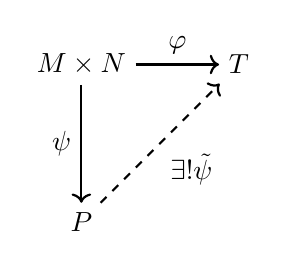
\begin{tikzpicture}[
    node distance=2cm,
    every node/.style={align=center}
]

% Nodes
\node (MxN) {$M \times N$};
\node (T) [right of=MxN] {$T$};
\node (P) [below of=MxN] {$P$};

% Arrows
\draw[->, thick] (MxN) -- node[above] {$\varphi$} (T);
\draw[->, thick] (MxN) -- node[left] {$\psi$} (P);
\draw[->, thick, dashed] (P) -- node[below right] {$\exists ! \tilde{\psi}$} (T);

\end{tikzpicture}
}

\thm{Existenz und Eindeutigkeit}{
    Für je zwei $R$-Moduln $M,N$ exestiert ein Tensorprodukt. Dieses ist bis auf eindeutige Isomorphie eindeutig bestimmt es gilt:

    \begin{equation}
        M \otimes_R N
    \end{equation}
}

\pf{}{
    \textbf{Existenz:} Sei $F$ der freie $R$-Modul mit Basis $((m,n))_{(m,n) \in M \times N}$. Damit sind die Elemente endliche $R$ Linearkombination von Elementen aus $M \times N$. Betrachte nun den Untermodul $U$ der von folgenden Elementen erzeugt wird.

    \begin{align}
        (m + m',n) - (m,n) - (m',n) \\
        (m,n + n') - (m,n) - (m,n') \\
        (rm,n) - r(m,n) \\
        (m,rn) - r(m,n)
    \end{align}

    Dabei gilt $m,m' \in M; n,n' \in N, r \in R$ nun ist $F/U$ ein Tensorprodukt und sehen dass folgende Abbildung bilinear ist.

    \begin{align}
        \varphi: M \times N \to F/U \\
        (m,n) \to (m,n) + U
    \end{align}

Sei nun $\psi: M \times N \to P$ eine weitere R-Bilineare Abbildung wir erhalten zunächst eine wohldefinierte Lineare Abbildung durch

\begin{align}
    \Psi: F \to P \\
    (m,n) \to \psi(m,n)
\end{align}

Aufgrund der Bilinearität liegt $U$ im Kern von $\Psi$ damit gibt es den Morphismus

\begin{align}
    \tilde{\psi} : F/U \to P \\
    (m,n) + U \to \psi(m,n)
\end{align}
wo offensichtlich $\psi = \tilde{\psi} \circ \varphi$ gilt. Durch die Bedingung ist $\tilde{\psi}$ auch eindeutig bestimmt mit Elementen $F/U$ und $\varphi(m,n) = (m,n) +U$

 \textbf{Eindeutigkeit:} Dazu betrachtet man einfach zwei Tensorprodukte

 \begin{equation}
     \varphi_1: M \times N \to T_1 \land \varphi_2: M \times N \to T_2
 \end{equation}

Nun ist $\varphi_2$ bilinear damit $\exists! f:T_1 \to T_2$ mit $\varphi_2 = f \circ \varphi_1$. Umgekehrt gibt es auch $g: T_2 \to T_1$ mit $\varphi_1 = g \circ \varphi_2$

\usetikzlibrary{arrows.meta}
\[
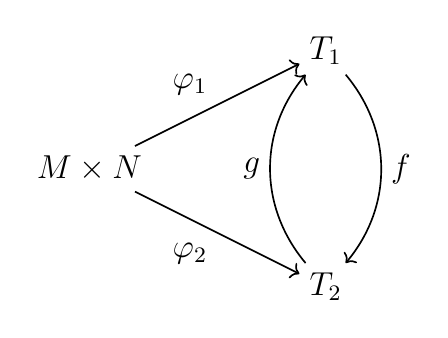
\begin{tikzpicture}[->, auto, node distance=2cm, semithick]
  \tikzstyle{every node}=[font=\large]
  \node (MN) at (0,0) {\( M \times N \)};
  \node (T1) at (3,1.5) {\( T_1 \)};
  \node (T2) at (3,-1.5) {\( T_2 \)};

  \draw[->] (MN) -- (T1) node[midway, above left] {\( \varphi_1 \)};
  \draw[->] (MN) -- (T2) node[midway, below left] {\( \varphi_2 \)};
  \draw[->, bend left=40] (T1) to node[midway, right] {\( f \)} (T2);
  \draw[->, bend left=40] (T2) to node[midway, left] {\( g \)} (T1);
\end{tikzpicture}
\]

}


\nt{Die Restklassen $(m,n) + U$ des Tensors bezeichnet man mit $m \otimes n$ und nennt sie \textbf{Elementartensor}. Es ist jedoch nicht jedes Element in $M \otimes_R N$ ein Elementartensor man muss auch Summen zulassen

    \begin{equation}
        M \otimes_R N = \{ \sum_{i=1}^d m_i \otimes n_i | d \in \NN, m_i \in M, n_i \in N \}
    \end{equation}

Wichtig sind hier die Rechenregeln welche aus der Konstruktion hervorgehen:

\begin{align}
    (m + m') \otimes n = m \otimes n + m' \otimes n \\
    m \otimes (n+ n') = m \otimes n + m  \otimes n' \\
    (rm) \otimes n  = r (m \otimes n) = m \otimes (rn)
\end{align}
}

\ex{}{Wir betrachten noch einige konkretere Tensorprodukte

    \begin{itemize}
        \item Beispielswiese gilt  $R^m \otimes_R R^n \cong Mat_{m,n} (R) \cong R^{mn}$ indem man die Abbildung $R^m \times R^n \to Mat_{m,n}(R); (v,t) \to vw^t$ betrachtet 
        \item Ähnlich gilt $R[x] \otimes_R R[y] \cong R[x,y]$
    \end{itemize}
}    
% subsection tensorprodukt (end)

\subsection{Ganze Ringerweiterungen und Hilberts Nullstellensatz} % (fold)
\label{sub:ganze_ringerweiterungen_und_hilberts_nullstellensatz}

Nun verallgemeinern wir den Begriff einer algebraischen Körpererweiterung auf Ringe. Problem an den Gleichungen in der Körpertheorie ist dass man diese meist normiert indem man durch den Leitkoeffizienten eines Polynoms dividiert. Dies ist in Ringen allgemein nicht möglich deshalb muss man die Normiertheit vorraussetzen. \emph{Anstelle von algebraisch spricht man hier von ganz}

\dfn{Ganzheitsgleichung, ganz über}{

    Sei $R \subset S$ eine Ringerweiterung

    \begin{enumerate}
        \item Ein Element $b \in S$ heißt  \textbf{ganz über R} falls $a_0,...,a_{n-1} \in R$ exestieren mit  $a_0 + a_1b +... + a_{n-1}b^{n-1} + b^n = 0$
             \item S heißt \textbf{ganz über R} falls jedes Element $b \in S$ ganz über R ist.
    \end{enumerate}
}

\thm{Charakterisierung von ganzen Ringwerweiterungen}{ Sei $R \subset S$ eine Ringerweiterung und  $b_1,...,b_m \in S$. Dann sind folgende Aussagen äquivalent:

    \begin{enumerate}
      \item $b_1,...,b_m$ sind ganz über R
      \item  $R[b_1,..,b_m]$ ist als R Modul endlich erzeugt
      \item $R[b_1,...,b_m]$ ist ganz über R
    \end{enumerate}
}
\pf{}{$(i) \implies (ii)$ Durch Auflösen einer Ganzheitsgleichung für $b_1$ nach $b_1^n$ gilt 

    \begin{equation}
        b_1^n = -(a_{n-1}b_1^{n-1}+...+a_0)
    \end{equation}
    
    für gewisse $a_i \in R$. Man kann die  $n$-te Potenz von  $b_1$ also immer durch niedrigere Potentzen von  $b_1$ und Koeffizienten aus  $R$ ersetzen. Man sieht also das  $R[b_1,...,b_m]$ von endlich vielen Produkten  $b_1^{e_1}...b_m^{e_m}$ erzeugt wird.

    $(ii) \implies (iii)$ Da endlich viele Elemente  $1 = c_1,...,c_n$ den R Modul $M:=R[b_1,...,b_m]$ erzeugen kann man $c \in M$ wählen und da  $M$ ein Ring ist auch  $c*c_i \in M$ und es gibt  $a_{ij} \in R$ mit 

     \begin{equation}
     c * c_i = \sum_{j=1}^{n} a_{ij}c_j
    \end{equation}

    Für die Matrix $A = (a_{ij})_{i,j} \in Mat_n(R)$ gilt dann 

     \begin{equation}
         A (c_1,...c_n)^T = c(c_1,...c_n)^T
    \end{equation}

    und es liegt $(c_1,...,c_n)^T$ im Kern von  $N:= cI_n - A$. Durch die Formel

     \begin{equation}
        det(N) \cdot (c_1,...,c_n) = 0
    \end{equation}

    folgt dann $det(N) = 0$ was aus der Leibnitzformel

    \begin{equation}
        det(N) = c^n + a_{n-1}c^{n-1} + ... + a_m
    \end{equation}

    eine Ganzheitsgleichung liefert
}

\thm{Hilberts Nullstellensatz, körpertheoretische Form}{
        Sei $k \subset K$ eine Körpererweiterung und  $K$ sei als Ring über  $k$ endlich erzeugt. Dann ist die Erweiterung  $k \subset K$ endlich und damit algebraisch
    }

\pf{}{
    Es gibt $\alpha_1,...,\alpha_n \in K$ mit $K = k[\alpha_1,...,\alpha_n]$. Wir beweisen die Aussage per Induktion über n.
    Im Fall $n=1$ gilt  $K=k[\alpha]$ dies ist ein Körper damit gibt es ein Polynom $p \in k[t]$ mit  $\alpha^{-1} = p(\alpha)$ i Daraus folgt $\alpha p(\alpha) - 1 = 0$ was eine algebraische Gleichung ist. Damit ist die Erweiterung algebraisch, endlich.
    Im Fall  $n-1 \to n$ betrachte $K= k(\alpha_1)[\alpha_2,...,\alpha_n]$ denn K ist ein Körper nun sind nach Induktionsannahme $\alpha_2,...,\alpha_n$ algebraisch über $k(\alpha_1)$ man zeigt nun dass $\alpha_1$ algebraisch über k ist. Dann ist die gesamte Erweiterung algebraisch und damit endlich.

Nun sind $\alpha_2,...,\alpha_n$ algebraisch über $k(\alpha_1)$ erfüllen also:

\begin{equation}
    u_i \alpha_i^d + \sum_{j=0}^{d-1}r_{ij}\alpha_i^j = 0
\end{equation}

mit $u_i,r_{ij} \in k[\alpha_1]$ man definiert nun $u := u_2 *** u_n \in k[\alpha_1]$ nun sind $\alpha_2,...,\alpha_n$ ganz über den Ring $k[\alpha_1,1/u]$ und es ist $K$ eine ganze Ringerweiterung von $k[\alpha_1,1/u]$. Angenommen $\alpha_1$ ist transzendent sprich $k[\alpha_1] \cong k[t]$ dann könne wir ein irreduzibles Polynom $p \in k[\alpha_1]$ wählen mit $p \nmid u$. Dann gibt es auch für  $p^{-1}$ eine Ganzheitsgleichung

\begin{equation}
    p^{-m} + b_1p^{-(m-1)} + ... + b_m = 0
\end{equation}

Multiplikation mit $p^m$ in einer genügend hohen Potenz und mit  $u$ liefert

\begin{equation}
    u^r + a_1p + ... + a_mp^m = 0
\end{equation}

was zeigt $p \nmid u$ ein Widerspruch und es ist nicht transzendent sondern algebraisch.

}

\cor{}{Sei $R$ als Ring über $k$ endlich erzeugt und $m$ ein maximales Ideal in $R$ dann ist $R/m$ eine endliche Körpererweiterung}

\pf{}{Es ist $R/m$ als Ring über $k$ immer noch endlich erzeugt und andererseits ein Körper.}

\cor{Hilberts Nullstellensaz, geometrische Form}{ Sei $k$ ein algebraisch abgeschlossener Körper und $I \lhd k[x_1,...,x_n]$ ein echtes Ideal. Dann exestiert ein $a \in k^n$ mit $p(a) = 0$ für alle $p \in I$. \emph{Damit hat das von I definierte polynomiale Gleichungsystem über k eine Lösung}}

\pf{}{Wähle ein maximales Indeal $m$ von $k[x_1,...,x_n]$ mit $I \subset m$. Nach Korrollar ist $k[x_1,...,x_n]/m$ eine endliche Körpererweiterung von $k$. Nun ist $k$ algebraisch abgeschlossen damit gilt $k[x_1,...,x_n]/m = k$. Setze nun $a_i := \bar{x_i}$ die Restklasse von $x_i$. Für jedes $p \in k[x_1,..,x_n]$ gilt dann 

    \begin{equation}
        p(a) = p(\bar{x}) = \bar{p}
    \end{equation}

damit gilt für $p \in I$ klarer Weise $p(a) = 0$}


% subsection ganze_ringerweiterungen_und_hilberts_nullstellensatz (end)

\section{Cyclotromic Polynomials} % (fold)
\label{sec:cyclotromic_polynomials}

This section should give a small revision of cylcotromic polynomials


% section cyclotromic_polynomials (end)



\section{Quaterionen} % (fold)
\label{sec:quaterionen}

\dfn{Quaterionen}{Seien $K$ ein Körper und $a,b\in K \setminus\{0\}$ Der Ring der Quaterionen $Q_K(a,b)$ is der $K^4$ mit den Basisvektoren

    \begin{equation}
    1,i,j,k
    \end{equation}
    Mit den Multiplikationsregeln
    \begin{equation}
    ij = k= -ij, i^2 = a*1, j^2 = b*1    
    \end{equation}
}
Diese oben definierte Rechenregel gibt uns eine Ringstruktur auf $K^4$ dabei ist der erste Basisvektor das neutrale Element es ergeben sich weitere Multiplikationsregel automatisch

\begin{equation}
ik = iij = a1 j = aj
\end{equation}

Oft schreibt man anstatt des Tuples $(v,w,x,y)$ auch die Vektorenschreibweise
\begin{equation}
v  + wi + xj + yk
\end{equation}

\dfn{Konjugierte Elemente und  Norm}{
    Für eine Element $p = v + swi + xj + yk \in Q_K(a,b)$ der Quaterionen definieren wir das konjugierte Element als 
    \begin{equation}
        \bar{p}:= v - wi - xj - yk \in Q_K(a,b)
    \end{equation}
    und die Norm 
    \begin{equation}
        N(p):= p \bar{p} = v^2 - aw^2 - bx^2 +aby^2 \in K
    \end{equation}
}
\mlemma{}{
\begin{enumerate}
    \item Für $p, q \in Q_K(a,b)$ gilt $\bar{pq} = \bar{q}\bar{p}$ 
    \item Für $p,q \in Q_K(a,b)$ gilt $N(pq) = N(p) N(q)$
    \item Es gilt $p \in Q_k(a,b)^\times \Leftrightarrow N(p) \neq 0$
\end{enumerate}
}
\pf{}{
    \begin{enumerate}
      \item Kann man einfach nachrechnen und sieht dann die Aussage sofort
      \item $N(pq) = pq\bar{pq} = pq\bar{q}\bar{p} = pN(q)\bar{p} = N(p)N(q)$ dies geht da $N(q) \in K \subset Z(Q_K(a,b))$
      \item Aus $pq = 1$ folgt $1 = N(1) = N(pq) = N(p)N(q)$ und daraus $N(p) \neq 0$ gilt umgekehrt
          das $N(p) \neq 0$ so setzen wir $q = \frac{1}{N(p)}\bar{p}$ dann ist $pq = 1$      
    \end{enumerate}
}

\thm{}{Sei $char(K) \neq 2$
\begin{enumerate}
  \item $Q_K(a,b)$ ist einfach
  \item Für jeden Teilkörper $K \subset \RR$ ist $Q_K(-1,-1)$ ein Schiefkörper
  \item Für $0 \neq b \in K$ gilt $Q_K(1,b) \cong Mat_2(K)$ insbesondere ist $Q_K(1,b)$ kein Schiefkörper
\end{enumerate}
}

\pf{}{
    Für (i) stellt man fest dass der Quaterionenring eine $K$-Algebra bildet man zeigt dann $Z(A)=K$ damit ist diese Algebra zentral. Für (ii) betrachtet man ein Element $0 \neq(v,w,x,w) \in K^4$ und stellt fest:
    \begin{equation}
    v^2 -(-1)w^2 -(-1)x^2 + (-1)(-1)y^2 = v^2 + w^2 + x^2 +y^2 \neq 0
    \end{equation}
    Für (iii) betrachtet man den Isomorphismus:
    \begin{align}
    Q_K(1,b) \to Mat_2(K) \\
    i \to
    \begin{pmatrix}
        1 & 0 \\
        0 & -1
    \end{pmatrix} \\
    j \to
    \begin{pmatrix}
        0 & b \\
        1 & 0
    \end{pmatrix}
    \end{align}
}

\section{Algebren} % (fold)
\label{sec:algebren}

In diesem Abschnitt sei nun $K$ ein Körper. Eine $K$-Algebra ist im Grunde ein Vektorraum in welchen multipliziert werden darf. Alternativ kann man es als Ring mit skalaren Multiplikation definieren

\dfn{K-Algebra und K-Unteralgebra}{
    \begin{itemize}
      \item Eine $K$-Algebra ist ein Ring $A$ zusammen mit einem Ringhomomorphismus $K \to Z(A)$
          \item eine $K$-Unteralgebra der $K$-Algebra $A$ ist ein Teilring $B \subset A$ der das Bild von K unter dem Homomorphismus erhält.
    \end{itemize}
}

\ex{}{
    \begin{itemize}
      \item Man kann also Elemente von $K$ mit Elementen von $A$ multiplizieren und erhält Elemente von $A$ als Ergebnis. Damit bildet $A$ einen K-Vektorraum. Gleichzeitig kann man aber auch zwei ELemente aus $A$ miteinander Multiplizieren da $A$ ein Ring ist. 
          \item Der Matrixring $Mat_m(K$ wird zu einer $K$-Algebra indem man Elemente von $k$ als Konstante Diagonalmatrizen der Größe $m$ auffasst.
          \item Der Polynomring $K[t]$ ist eine Kommutative $k$-Algebra.
              \item Der Quaterionenring $Q_K(a,b)$ ist eine $K$-Algebra.
    \end{itemize}
}
Im folgenden betrachten wir Unteralgebren von Matrix-Algebren. Für eine $K$-Unteralgebra $A \subset Mat_m(K)$ nennt man einen Untervektorraum \textbf{invariant} falls $Mv \in K$ gilt 

\thm{Satz von Burnside}{
    Sei $K$ ein algebraisch abgeschlossener Körper. Falls die $K$-Unteralgebra $A \subset Mat_m(K)$ nur die beiden trivialen invarianten Unterräume besitzt gilt $A=Mat_m(K)$ 
}
\pf{}{
    A operiert transitiv auf $K^m$: für jedes  $0 \neq v \in K^m$ ist

    \begin{equation}
        \{0 \} \subset \{ Mv | M \in A \}
    \end{equation}
    ein $A$ invarianter Unterraum stimmt also mit $K^m$ überein. Nun zeigt man das $A$ eine Matrix vom Rang 1 enthält. sei $0 \neq P \in A$ falls $rang(P) \geq 2$ ist wähle $v_1,v_2 \in K^m$ mit $Pv_1, Pv_2$ linear unabhängig.

    Wähle dann $MPv_1 = v_2$ das geht da A transitiv operiert. Dann ist $PMPv_1$ und $Pv_1$ linear unabhängig es gilt $PMP-\lambda P \neq  0$ für alle $\lambda in K$. Nun gibt es ein $\lambda_0 \in K$ sodass $PM - \lambda_0 I_d$ auf den Raum $P(K^m)$ nicht invertierbar ist, denn K ist algebraisch abgeschlossen und jede lineare Abbildung hat einen Eigenwert.

    \begin{equation}
        (PM-\lambda_0 I_d)P
    \end{equation}
    hat echt kleineren Rang als $P$, ist aber nicht Null. Iterativ erhält man also eine Matrix $Q$ vom Rang 1 in A. Dann ist jedoch auch jede beliebige Rang 1 Matrix in A und es gilt $A = Mat_m(K)$

}

\ex{}{Sei $A \subset Mat_m(\mathbb{C})$ sogar eine $*$-Unteralgebra, dh mit $M$ gehört auch $M^*$ zu A. Falls $A$ einen echten invarianten Unterraum $V \subset \mathbb{C}^m$ besitzt, so ist auch  $V^\perp$ ein solcher invarianter Unterraum. Man verwendet das $A$ abgeschlossen unter $*$ ist nach einen unitären Basiswechsel haben alle Matrizen in $A$ Blockgestalt damit gilt

    \begin{equation}
        Mat_{m_1}(\mathbb{C}) \oplus Mat_{m_2}(\mathbb{C})
    \end{equation}

}

\dfn{Zentral}{
    Eine $K$-Algebra $A$ heißt zentral, wenn $Z(A)=A$ gilt
}

So ist beispielsweise für Körper  $K$,  $Mat_m(K)$ eine zentrale $K$-Algebra. Für $char(K)\neq 2$ ist $Q_K(a,b)$ eine zentrale $K$-Algebra.
% section algebren (end)

\section{Kodierungstheorie} % (fold)
\label{sec:kodierungstheorie}

Ziel der Kodierungstheorie ist es Daten so aufzubereiten dass Fehler welche bei der Übertragung gemacht werden erkannt und bestenfalls verbessert werden können.

\ex{ISBN-10}{ Die ISBN-10 Nummer eines Buchs besteht aus einer Zahl mit 10 Ziffern

    \begin{equation}
        x_1x_2...x_{10}
    \end{equation}
    Dabei tragen nur die ersten $9$ Ziffern wirkliche Information die $x_{10}$ ist eine Prüfziffer. Sie wird durch die folgende Prüfgleichung erfüllt:

    \begin{equation}
        x_1 + 2x_2 + 3x_3 + 4x_4 + 5x_5 + 6x_6 + 7x_7 + 8x_8 + 9x_9 + 10x_{10} = 0 \mod 11
    \end{equation}

    Dies kann man da $10=-1 \mod 11$ gilt umformen zu 

    \begin{equation}
        x_{10} = x_1+ 2x_2 ... + 9x_9 \mod 11
    \end{equation}

    Man macht hierbei folgende Beobachtungen

    \begin{itemize}
      \item Wird genau eine Ziffer einer gültigen ISBN-10 Nummer abgeändert, ist die Prüfgleichung nicht mehr erfüllt. Solch ein einfacher Fehler wird also immer endteckt.
          \item Wird genau eine Ziffer abgeändert, und weiß man um welche es sich handelt so kann sie aus der Prüfgleichung rekonstruiert werden
    \end{itemize}

    Um mehr Ziffern zu Vefügung zu haben wurde die  \textbf{ISBN-13} Nummer eingeführt diese besteht aus 13 Ziffern $x_1...x_{13}$ wobei nur $12$ Ziffern die eigentliche Information tragen und $x_{12}$ über die Prüfgleichung

    \begin{equation}
        x_1 + 3x_2 + x_3 + ... + x_{12} = 0 \mod 10
    \end{equation}
    bestimmt wird

}

\dfn{Alphabet, Code}{
    \begin{enumerate}
      \item Ein Alphabet $A$ ist eine endliche Menge
          \item Ein Wort über $A$ ist ein Tupel $x = (x_1,...,x_k) \in A^k$ dabei heißt $k$ die Wortlänge
              \item Eine Kodierungsregel ist eine injektive Abbildung $\varphi: A^k \to A^n$ für $k,n \in \NN$.
                  \item Für eine Kodierungsregel $\varphi: A^k \to A^n$ nennt man die Elemente von $A^k$ Informationswörter und $\varphi(x) \in A^n, x \in A^k$ nennt man Codewort. Die Menge $\varphi(A^k)$ aller Codewörter ist der Code
    \end{enumerate}
}

Die Idee ist also. Die Informationswörter tragen die eigentliche Information, die gespeichert und oder übermittelt werden soll, man erhält das Codewort. Aufgrund der \textbf{Injektivität} von $\varphi$ kann die eigentliche Infromation aus einem Codewort zurückermittelt werden.

\ex{}{
    FÜr den ISBN-10 Code ist $A = \mathbb{F}_{11}$ und 

    \begin{align}
        \varphi F_{11}^9 \to F_{11}^{10} \\
        (x_1,...,x_9) \to (x_1,...,x_9,x_{10})
    \end{align}
    

    Der $d$-Wiederholungscode hat die Kodierungsregel:

    \begin{align}
        \varphi: A^k \to A^{dk}
        (x_1,...,x_k) \to (x_1,...,x_k,x_1,....,x_k,x_1,....,x_k)
    \end{align}
}
\dfn{Hamming-Distanz}{
    Sei $A$ ein Alphabet und $n \in \NN$. Die Hamming Distanz zweier Elemente $v =(v_1,...,v_n), w= (w_1,...,w_n) \in A^n$ ist definiert durch

    \begin{equation}
        d(v,w) := \# \{i|1 \leq i \leq n, v_i \neq w_i \}
    \end{equation}

    \textbf{Die Hamming-Distanz ist eine Metrik auf $A^n$}

}

In der Praxis geht man also folgendermaßen vor: Es wird die Information $x \in A^k$ kodiert und das Codewort $\varphi(x) \in A^n$ versendet. Der Empfänger erhält dann ein Wort $r \in A^n$ dass aufgrund von Fehlern in der Übertragung von $\varphi(x)$ verschieden sein kann. Es sucht nun mit der Hamming Distanz das nächstgelegende Codewort $c = \varphi(y) \in \varphi(A^k)$ und schließt mit der Injektivität auf die ursprüngliche Information

\dfn{e-fehlerkorrigierend}{Sei $e \in \NN$ ein Code $C \subset A^n$ heißt  \textbf{e-fehlerkorrigierend} falls die abegschlossenen Bälle in $A^n$ mit Radius $e$ um Elemente von $C$ paarweise disjunkt sind.
}

Wird also bei einen Code $C$ der e-fehlerkorrigierend ist nur an $e$-Stellen ein Fehler gemacht dann liefert die Vorgehensweise die richtige Information zurück.

\dfn{Minimaldistanz von $C$}{
Für $C \subset A^k$ definieren wir die Minimaldistanz von $C$ als 

\begin{equation}
    d_{min}(C):= min\{d(v,w) | v,w \in C, v \neq w \}
\end{equation}
}

\mlemma{}{Ein Code mit Minimaldistanz $d$ ist genau dann  $e$-fehlerkorrigierend, wenn $e \leq [ \frac{d-1}{2}]$ gilt}

Die Minimaldistanz des $d$ Wiederhilungscodes ist gerade $d$ fpr $d=2e+1$ ist dieser Code also $e$ fehlererkennend. Wenn man also bei der Kodierung $e$ fehler gemacht hat so müssen $d-e = 2e+1 - e = e+1$ der Wiederholungen übereinstimmen.

\dfn{Linearer (n,k)-Code}{
    EIn linearer (n,k) Code über $\mathbb{F}_q$ ist ein $k$ dimensionaler $F_q$ Untervektorraum von $\mathbb{F}_q^n$
}

% section kodierungstheorie (end)

\section{Kryptographie} % (fold)
\label{sec:kryptographie}

Man möchte hier eine Nachricht so verschlüsseln das man sie einen Empfänger zukommen lassen kann, ohne das ein eventuell unerwünschter Zuhörer den Inhalt versteht. Man verschlüsselt also die eigentliche Information der Empfänger muss die Nachricht dann wieder entschlüsseln.

\textbf{Cäsar Verschlüsselung} die Idee hierbei ist das sich Senderin Alice (A) und Empfänger Bob (B) eine Ersetzungsregel für Buchstaben ausdenken. Jeder Buchstabe der eigentlichen Nachricht (Klartext) wird in Geheimtext verschlüsselt 

\begin{equation}
    a \to d, b \to j x \to t ... 
\end{equation}

Wird dabei nur eine Verschiebung von Buchstaben verwendet kann man dies durch probieren aller 26 Möglichkeiten sehr einfach lösen. Hat die dritte Person Eve keine Kenntnis über die verwendete Ersetzungsregel so gibt es 

\begin{equation}
    26! \sim 2^{88}
\end{equation}

mögliche Kombinationen, was nicht möglich ist. Knacken kann man diesen Code jedoch durch \textbf{Häufigkeitsanalyse} so kommen die Buchstaben in verschiedenen Sprachen in unterschiedlicher Häufigkeit vor. In Deutsch sind beispielsweise $e, n,i$ häufig vorkommende Buchstaben. Durch das Zuordnen diesr kann der Code dann geknackt werden.

Um dieses Problem zu umgehen werden meist  \textbf{Vigenere Verschlüsselungen} verwendet hier bekommt jeder Buchstabe eine eigene Ersetzungsregel. Es vereinbaren Alice und Bob dann ein Schlüsselwort (z.b BACH)

\begin{itemize}
  \item Erster Buchstabe wird mit zweiter Zeile verschlüsselt
      \item Zweiter Buchstabe wird mit erster Zeile verschlüsselt
          \item Dritter Buchstabe wird mit dritter Zeile verschlüsselt
\end{itemize}

Man wiederholt dieses Verfahren mit dem gesamten Klartext, hier versagt die klassische Häufigkeitsanalyse komplett. Man kann, falls das Schlüsselwort eher kurz ist jedoch eine andere Taktik verwenden. So gibt es in jeder Sprache einige kurze Wörter die relativ häufig vorkommen, im Deutschen beispielsweise "und", "der", "die. Es kommen in diesem Fall mit einger Wahrscheinlichkeit eines dieser Worter in einen Abstand vor der ein vielfaches der Schlüsselwortlänge ist. Dann wendet man auf die kurzen Buchstabenketten im Geheimtext die Häufigkeitsanalyse an.

\emph{Ist der Geheimtext und das Schlüsselwort jedoch gleich lang so ist der Code in der Tat unknackbar!}

\textbf{Diffie-Hellmann-Verfahren} ist ein Pulic Key Verfahren hier können $A$ und $B$ über einen unsicheren Kanal Informationen austauschen. Es kommt zu einer Erstellung eines Schlüssels den $E$ nicht kennt.

\begin{itemize}
  \item Alice und Bob vereinbaren öffentlich eine Primzahl $p$ und ein Element $g \in \ZZ / p \ZZ$
  \item Alice wählt eine Zahl $a \in \{1,...,p-1 \}$ die sie geheim hält.
  \item Bob wählt eine Zahl $b \in \{1,...,p-1\}$ die er geheim hält.
      \item Alice sendet Bob $g^a \in \ZZ / p \ZZ$
          \item Bob sendet Alice  $g^b \in \ZZ / p \ZZ$
          \item Sowohl Alice als auch Bob können über $(g^a)^b = (g^b)^a = g^{ab}$ den Code entschlüsseln
\end{itemize}


Möchte Eve nun $g^{ab}$ bestimmen so muss sie den Logarithmus zur Basis $g$ von $g^a$ ausrechnen. Normal ist dies kein Problem und kann durch ein Schachtelungs-Algorithmus erledigt werden. Problematisch ist nur das die Exponentialfunktion in $(\ZZ / p\ZZ)^\times$ ein Sprungverhalten zeigt und die Berechnung ist für großes $p$ praktisch unmöglich. In der Praxis verwendet man auch gerne den Körper der elliptischen Kurven:

\dfn{Elliptische Kurve}{
    Seien $r,s \in K$ dann heißt die Menge

    \begin{equation}
        C = \{(a,b) \in \bar{K}^2 | b^2 = a^3 + ra + s \}
    \end{equation}
    eine elliptische Kurve über K. Falls für einen Punkt $(a,b) \in C$ sogar $a,b \in K$ gilt so heißen $(a,b)$ ein rationaler Punkt der Kurve
}

% section kryptographie (end)


\section{Kategorientheorie} % (fold)
\label{sec:kategorientheorie}

\dfn{Kategorie}{
    Eine \textbf{Kategorie} $C$ besteht aus eine Klasse

    \begin{equation}
        Obj(C)
    \end{equation}
    von sogenannten Objekten und für alle  $X,Y \in Obj(C)$ jeweils aus einer Menge von Morphismen

    \begin{equation}
        C(X,Y)
    \end{equation}
    und partiellen Verknüpfungen von Morphismen

    \begin{align}
        C(X,Y) \times C(Y,Z) \to C(X,Z) \\
        (f,g) \to g \circ f
    \end{align}

    diese erfüllen jeweils zwei Bedingungen:

    \begin{enumerate}
      \item $\forall X \in Obj(C) \exists id_X \in C(X,X)$ mit $id_x \circ f = f, g \circ id_x = g$ für alle $f \in C(Y,X), g \in C(X,Y)$
           \item Für alle $f \in C(W,X), g\in C(X,Y), h \in C(Y,Z)$ gilt $h \circ (g \circ f) = (h \circ g) \circ f$ 
   \end{enumerate}
  Man nennt $f \in C(X,Y)$ einen Isomorphismus, falls $g \in C(Y,X)$ exestiert mit $g \circ f = Id_x, f \circ g = id_Y$
}

Ausschnitte aus den Kategorien stellt man gewöhlich durch kommutative Pfeildiagramme dar, unten gezeigt die Komposition von Morphismen.
\usetikzlibrary{arrows.meta, positioning}
\[
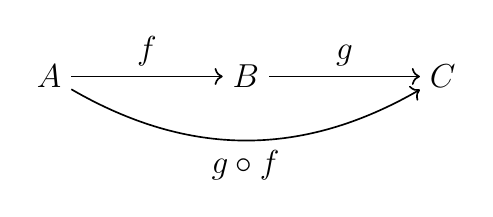
\begin{tikzpicture}[->, node distance=2.5cm, semithick]
  \tikzstyle{every node}=[font=\large]
  \node (A) {\( A \)};
  \node (B) [right of=A] {\( B \)};
  \node (C) [right of=B] {\( C \)};

  \draw[->] (A) -- (B) node[midway, above] {\( f \)};
  \draw[->] (B) -- (C) node[midway, above] {\( g \)};
  \draw[->, bend right=30] (A) to node[midway, below] {\( g \circ f \)} (C);
\end{tikzpicture}
\]

\ex{}{
    \begin{itemize}
      \item Die Kategorie $Men$ hat also Objekte die Mengen und als Morphismen die Abbildungen. Die Verknüpfungen sind hier die Hintereinanderausführungen
          \item Für jeden festen Körper $K$ gibt es die Kategorie $K-Vec$ der Vektorräume hier sind die Morphismen die $K$-linearen Abbildungen
              \item Die Kategorie $Top$ der topologischen Räume hat als Morphismen die stetigen Abbildungen. Hier wird der Isomorphismus gerade Homöomorphismus genannt.
    \end{itemize}
}



\dfn{Kovarianter und Kontravarianter Funktor}{
    Ein \textbf{kovarianter bzw. kontravarianter} Funktor von der Kategorie $C$ in die Kategorie $D$ besteht aus einer Abbildung

     \begin{equation}
        F: Obj(C) \to Obj(D)
    \end{equation}

und jeweils Abbildungen

\begin{align}
    F: C(X,Y) \to D(F(X), F(Y)) \\
    F: C(X,Y) \to D(F(Y),F(X))
\end{align}

mit

\begin{itemize}
    \item $F(id_X) = id_{F(x)}$ 
        \item $F(g \circ f) = F(g) \circ F(f)$
             \item $F(g \circ f) = F(f) \circ F(g)$
\end{itemize}
}


\ex{}{
    \begin{itemize}
      \item Die Bildung des Dualraums ist ein kontravarianter Funktor von $K-Vec$ in sich selbst
          \item Sei X ein fest gewählter $K$-Vektorraum. Dann ist die Zuordnung $V \to X \otimes V$ ein kovarianter Funktor von  $K-Vec$ in sich selbst. Dabei wird eine lineare Abbildung $\varphi: V \to W$ auf $id_X \otimes \varphi: X \otimes V \to X \otimes W$ abgebildet
              \item Es gibt kovarianten Funktor $Top \to Men$ der jedem topologischen Raum die Menge seiner Zusammenhangskomponenten abbildet. Stetige Abbildungen erhalten den Zusammenhang
                  \item Es gibt den kovarianten Vergiss Funktor $C \to Men$ der eventuelle Zusatzstruktur auf den Objekten der Kategorie einfach vergisst.
    \end{itemize}
}

\mlemma{}{
    Sei $F: C \to D$ ein Funktor und in $C$ gelte $X \cong Y$ Dann gilt in $D$
     \begin{equation}
        F(X) \cong F(Y)
    \end{equation}
}

\pf{}{Sei o.B.d.A $F$ kovariant. Sei $f \in C(X,Y)$ ein Isomorphismus mit $g in C(Y,X)$ und $g \circ f = id_X$ nach Anwendung des Funktors:

    \begin{equation}
        id_{F(x)} = F(id_X) = F(g \circ f) = F(g) \circ F(f)
    \end{equation}
    Analog bekommt man $F(f) \circ F(g) = id_{F(Y)}$ und die gewünschte Aussage
}

\section{Garbentheorie} % (fold)
\label{sec:garbentheorie}

\dfn{Ring-Prägarbe}{
    Sei $X$ ein topologischer Raum. Eine \textbf{Ring-Prägarbe} $F$ auf $X$ besteht aus den Daten:

    \begin{itemize}
        \item Für jede offene Teilmenge $U \subset X$ einen Ring $F(U)$ wobei $F(\emptyset) = \{0 \}$ 
        \item Für je zwei offene Teilmengen $U \subset V$ einen Ringhomomorphismus $r_{V,U}: F(V) \to F(U)$
    \end{itemize}

Diesen Ringhomomorphismus nennt man  \textbf{Restriktion von $V$ auf $U$} dabei gilt für drei offene Mengen $U \subset V \subset W$ stets

\begin{equation}
    f_{V,U} \circ r_{W,V} = r_{W,U}
\end{equation}

und $r_{U,U} = id_{F(U)}$
}

\ex{}{Seien $X,W$ zwei topologische Räume. Für $U \subset X$ offen sei $C(U,W)$ die Menge aller stetigen Funktionen von $U$ nach $W$. Wiederum mit den Restriktionen von Funktionen auf kleinere Definitionsbereiche erhalten wir eine Prägarbe  $C$ auf $X$.}

Um nun die \emph{Lokalität} der Bedingung an den Funktionen axiomatisch zu erfassen definiert man den Begriff einer Garbe.

\dfn{Garbe}{
    Sei $X$ ein topologischer Raum. Eine \textbf{Garbe} auf X ist eine Prägarbe $F$ die zusätzlich folgende Bedingung erfüllt: 

    FÜr jedes offene $U \subset X$, jede offene Überdeckung $U = \bigcup_{i \in I U_i}$ und jede Auswahl von Elementen $s_i \in F(U_i)$ mit 

        \begin{equation}
            r_{U_i, U_i\cap U_j}(s_i) = r_{U_j, U_i\cap U_j}(s_j)
        \end{equation}

        für alle $i,j \in I$ gibt es genau ein $s \in F(U)$ mit $r_{U,U_i}(s) = s_i, \forall I$ 
    }

    Denkt man sich die $F(U)$ jeweils als Menge von auf $U$ definierten Funktionen, so sagt die Garbeneigenschaft, dass die Bedingung an die betrachteten Funktionen \textbf{lokal} ist. Für vorgegebene Funktionen $s_i$ auf $U_i$ welche auf paarweisen Schnitten übereinstimmen gibt es genau eine global auf $U$ definierte Funktion $s$ die alle $s_i$ fortsetzt. Dieses $s$ muss nun automatisch auf die Bedingung in $F$ erfüllen.

    Ein konkretes Beispiel ist die Garbe $C$ mit stetigen Funktionen zwischen topologischen Räumen. Auf die Einschränkung $F_{|U}$ einer Garbe auf eine offene Teilmenge $U \subset X$ ist offensichtlich wieder eine Garbe.

\dfn{Morphismus von Garben}{
    Seien $(X,F), (Y,G)$ topologische Räume mit Garben. Ein Morphismus von Garben besteht aus den Daten

    \begin{itemize}
      \item Stetige Abbildung $f: X \to Y$ 
        \item    Für jede offene Menge $U \subset Y$ einen Ringhomomorphismus $f^*_U: G(U) \to F(f^{-1}(U))$
    \end{itemize}
}

Man nennt hier die Abbildung $f_U^*$ auch die Zurückziehung von Elementen aus $G(U)$ nach $F(f^{-1}(U)$. Sind $X,Y$ topologische Räume mit der Garbe der Stetigen Funktionen mit Werten in $W$ dann erhält man fpr jede stetige Funktion $f: X \to Y$ einen Morphismus indem man $f^*$ als Zurückziehung mittels $f$ definiert

\dfn{Halm}{
    Um das lokale Verhalten einer Garbe an einem Punkt zu erfassen, definiert man den Begriff eines Halms. Sei $(X,F)$ eine  (Prä)-Garbe und $x \in X$. Auf der Menge

    \begin{equation}
        M:= \{(U,s) | x \in U, U \subset X ~ offen, s \in F(U) \}
    \end{equation}
    definiert man eine Äquivalenzrelation

    \begin{equation}
        (U,s) \sim (V,t) :\Leftrightarrow \exists W \subset U \cap V ~ offen, x \in W, r_{U,W}(s) = r_{V,W}(t)
    \end{equation}

    Konkret für Garben von Funktionen sagt dies das zwei auf Umgebungen von $x$ definierte Funktionen äquivalent sind wenn sie auf einer kleinen offenen Umgebung von $x$ übereinstimmen. Die Menge 

    \begin{equation}
        F_x := M/\sim = \{ [(U,s)] | (U,s) \in M \}
    \end{equation}
    der Äquivalenzklassen trägt eine kanonische Ringstruktur

    \begin{equation}
        [(U,s)] + [(V,t)] := [(U \cap V, r_{U,U \cap V}(s) + r_{V,U \cap V}(t))] 
    \end{equation}

    Dies nennt man dann Halm der Garbe $F$ am Punkt $x$

}

Für jedes $U \subset X$ mit $x \in U$ gibt es den kanonischen Homomorphismus

\begin{align}
    F(U) \to F_x \\
    s \to [(U,s)]
\end{align}

Weiteres ist $\varphi=(f,f^*): (X,F) \to (Y,G)$ ein Garbenmorphismus, so induziert er für jedes $x \in X$ einen kanonischen Morphismus der Halme

\begin{align}
    \varphi_x : G_{f(x)} \to F_x \\
    [(U,s)] \to [(f^{-1}(U), f^*(s)]
\end{align}

\thm{Isomorphismus der Halme}{
    Sei $\varphi (f,f^*): (X,F) \to (Y,G)$   ein Morphismus von Garben, wobei $f$ ein Homöomorphismus der topologischen Räume sei. Dann ist $\varphi$ genau dann ein Isomorphismus, wenn für alle $x \in X$ die induzierten Morphismen $\varphi_x$ der Halme Isomorphismen sind. 
}


% section garbentheorie (end)

\end{document}
